\documentclass[11pt,a4paper]{article}

% Image mode: pdf.
% Image paths stay relative. In PDF mode, place same-basename PDF conversions
% of the chapter SVG files in the assets/ directory beside this source.

\usepackage{iftex}
\ifPDFTeX
  \PackageError{handout}{This template requires XeTeX or Tectonic}{Compile with xelatex or tectonic.}
\fi

\usepackage[a4paper,top=18mm,bottom=20mm,left=20mm,right=20mm,headsep=6mm]{geometry}
\usepackage{fontspec}
\usepackage{xeCJK}
\usepackage{amsmath}
\usepackage{unicode-math}

% Font settings are intentionally visible in the generated .tex file.
% These defaults target the macOS machine used for the released PDF.
% Change the family names when compiling on another system.
\setmainfont{Songti TC}
\setsansfont{Heiti TC}
\setmonofont{Menlo}
\setCJKmainfont{Songti TC}
\setCJKsansfont{Heiti TC}
\setCJKmonofont{Heiti TC}
\setmathfont{STIX Two Math}
\XeTeXlinebreaklocale "zh"
\XeTeXlinebreakskip=0pt plus 1pt

\usepackage{xcolor}
\definecolor{HandoutBlue}{HTML}{215A91}
\definecolor{HandoutBlueLight}{HTML}{EEF5FC}
\definecolor{HandoutGreen}{HTML}{39715A}
\definecolor{HandoutGreenLight}{HTML}{EFF8F3}
\definecolor{HandoutGold}{HTML}{8A641C}
\definecolor{HandoutGoldLight}{HTML}{FFF8E8}
\definecolor{HandoutInk}{HTML}{253142}
\definecolor{HandoutMuted}{HTML}{667085}

\usepackage{graphicx}
\makeatletter
% Pandoc 3 emits an accessibility `alt` key for raster/PDF images. Older
% graphicx releases do not know that key, so accept it without changing layout.
\@ifundefined{KV@Gin@alt}{\define@key{Gin}{alt}{}}{}
\newsavebox\pandoc@box
\newcommand*\pandocbounded[1]{%
  \sbox\pandoc@box{#1}%
  \Gscale@div\@tempa{\textheight}{\dimexpr\ht\pandoc@box+\dp\pandoc@box\relax}%
  \Gscale@div\@tempb{\linewidth}{\wd\pandoc@box}%
  \ifdim\@tempb\p@<\@tempa\p@\let\@tempa\@tempb\fi
  \ifdim\@tempa\p@<\p@\scalebox{\@tempa}{\usebox\pandoc@box}%
  \else\usebox{\pandoc@box}%
  \fi
}
\makeatother
\usepackage{float}
\floatplacement{figure}{H}
% Pandoc uses LTcaptype=none for uncaptioned longtables. The caption package
% expects that name to exist as a counter even though it is never displayed.
\newcounter{none}
\usepackage{caption}
\captionsetup[figure]{labelformat=empty,labelsep=none,font=small}

\usepackage{booktabs,longtable,array,calc}
\usepackage{etoolbox}
\makeatletter
\patchcmd\longtable{\par}{\if@noskipsec\mbox{}\fi\par}{}{}
\makeatother

\usepackage[most]{tcolorbox}
\tcbuselibrary{breakable,skins}
\newtcolorbox{HandoutLearningMap}{
  enhanced,breakable,colback=HandoutBlueLight,colframe=HandoutBlue,
  boxrule=0.8pt,arc=1.5mm,left=3mm,right=3mm,top=2mm,bottom=2mm,
  before skip=8pt,after skip=10pt
}
\newtcolorbox{HandoutWorkedExample}{
  enhanced,breakable,colback=HandoutGreenLight,colframe=HandoutGreen,
  boxrule=0.65pt,arc=1.5mm,left=3mm,right=3mm,top=2mm,bottom=2mm,
  before skip=8pt,after skip=10pt
}
\newtcolorbox{HandoutSelfCheck}{
  enhanced,breakable,colback=HandoutGoldLight,colframe=HandoutGold,
  boxrule=0.65pt,arc=1.5mm,left=3mm,right=3mm,top=2mm,bottom=2mm,
  before skip=8pt,after skip=10pt
}

\usepackage{titlesec}
\titleformat{\section}{\sffamily\bfseries\Large\color{HandoutBlue}}{}{0pt}{}
\titleformat{\subsection}{\sffamily\bfseries\large\color{HandoutInk}}{}{0pt}{}
\titleformat{\subsubsection}{\sffamily\bfseries\normalsize\color{HandoutInk}}{}{0pt}{}
\titlespacing*{\section}{0pt}{1.4em}{0.55em}
\titlespacing*{\subsection}{0pt}{1.15em}{0.45em}
\titlespacing*{\subsubsection}{0pt}{0.9em}{0.35em}
\setcounter{secnumdepth}{-\maxdimen}

\usepackage{hyperref}
\usepackage{bookmark}
\IfFileExists{xurl.sty}{\usepackage{xurl}}{}
\urlstyle{same}
\hypersetup{
  colorlinks=true,
  linkcolor=HandoutBlue,
  urlcolor=HandoutBlue,
  citecolor=HandoutBlue,
  pdftitle={必物-5 能量},
  pdfsubject={物理},
  pdfcreator={Pandoc with the HighSchooContent LaTeX template}
}

\setlength{\parindent}{0pt}
\setlength{\parskip}{0.55em plus 0.15em minus 0.1em}
\setlength{\emergencystretch}{3em}
\setlength{\LTpre}{0.5em}
\setlength{\LTpost}{0.5em}
\renewcommand{\arraystretch}{1.18}
\providecommand{\tightlist}{%
  \setlength{\itemsep}{0pt}\setlength{\parskip}{0pt}}
\pagestyle{plain}


\begin{document}

\begin{tcolorbox}[
  enhanced,colback=white,colframe=HandoutBlue,boxrule=1.1pt,arc=2mm,
  borderline west={3pt}{0pt}{HandoutBlue},left=5mm,right=4mm,top=4mm,bottom=4mm
]
{\sffamily\small\bfseries\color{HandoutBlue}學生講義}\par
{\sffamily\bfseries\LARGE\color{HandoutInk}必物-5 能量}\par
\vspace{0.35em}{\large 用同一套能量帳連接機械運動、溫度、發電與核反應}\par
\vspace{0.45em}{\small\color{HandoutMuted}%
科目：物理
\quad 課程：普通高中必修物理
\quad 版本：學生版｜核心＋理解
\quad 校訂：2026-08-29
}\par
\vspace{0.25em}{\small\color{HandoutMuted}範圍：功與能量形式、微觀尺度能量、能量守恆與轉換、質能互換與核能}\par
\end{tcolorbox}


能量是跨尺度的計帳方法。物體加速、升高、摩擦升溫、電廠發電與核反應，看似是不同現象，都可先指定系統，再追蹤能量從哪裡進入、以什麼形式儲存、往哪裡移出。這套方法能分析煞車距離、遊樂設施速度、電器耗能、儲能效率與輻射安全。

本章採用下列約定：近地面重力場取 \(g=9.8\ \mathrm{m/s^2}\)；題目標示「取 \(g=10\ \mathrm{m/s^2}\)」時依題意計算。溫差可用 \(^\circ\mathrm C\) 或 K 表示；溫度的倍數關係使用 K。能量與功的 SI 單位都是焦耳（J），功率單位是瓦特（W），\(1\ \mathrm W=1\ \mathrm{J/s}\)。

\begin{HandoutLearningMap}

\subsection{本章問題與能力}\label{ux672cux7ae0ux554fux984cux8207ux80fdux529b}

\begin{enumerate}
\def\labelenumi{\arabic{enumi}.}
\tightlist
\item
  力經過一段位移時，如何由方向、距離或圖面積計算轉移的能量？
\item
  如何用動能、位能與內能描述宏觀運動及微觀粒子運動？
\item
  如何先選系統，再以守恆式追蹤摩擦、加熱、發電與儲能的每一筆能量？
\item
  如何用質量虧損、核子帳與輻射種類分析核反應及安全控制？
\end{enumerate}

\subsection{實際用途}\label{ux5be6ux969bux7528ux9014}

功---動能定理可估算煞車與加速，力學能可預測軌道速度，量熱與效率可估算熱水器耗電，多段能量帳可比較發電與儲能，質能關係及穿透模型可分析核能與輻射防護。

\end{HandoutLearningMap}

{\def\LTcaptype{none} % do not increment counter
\begin{longtable}[]{@{}
  >{\raggedright\arraybackslash}p{(\linewidth - 4\tabcolsep) * \real{0.3333}}
  >{\raggedright\arraybackslash}p{(\linewidth - 4\tabcolsep) * \real{0.3333}}
  >{\raggedright\arraybackslash}p{(\linewidth - 4\tabcolsep) * \real{0.3333}}@{}}
\toprule\noalign{}
\begin{minipage}[b]{\linewidth}\raggedright
問題
\end{minipage} & \begin{minipage}[b]{\linewidth}\raggedright
先確定的量
\end{minipage} & \begin{minipage}[b]{\linewidth}\raggedright
能量帳
\end{minipage} \\
\midrule\noalign{}
\endhead
\bottomrule\noalign{}
\endlastfoot
力使物體移動 & 力與位移的夾角 & \(W=Fs\cos\theta\) \\
速度或高度改變 & 初、末狀態與零位面 & \(K=\frac12mv^2\)，\(U_g=mgh\) \\
氣體溫度或粒子數改變 & 系統所含粒子與絕對溫度 & 溫度看平均動能，內能看總和 \\
摩擦、加熱或機器轉換 & 系統邊界與能量流 & \(E_i+E_{\mathrm{in}}=E_f+E_{\mathrm{out}}\) \\
核反應放能 & 反應前後總質量 & \(E=\Delta mc^2\) \\
\end{longtable}
}

\clearpage

\section{1　功、功率與能量形式}\label{ux529fux529fux7387ux8207ux80fdux91cfux5f62ux5f0f}

\subsection{1.1 功：力透過位移轉移能量}\label{ux529fux529bux900fux904eux4f4dux79fbux8f49ux79fbux80fdux91cf}

\begin{figure}
\centering
\pandocbounded{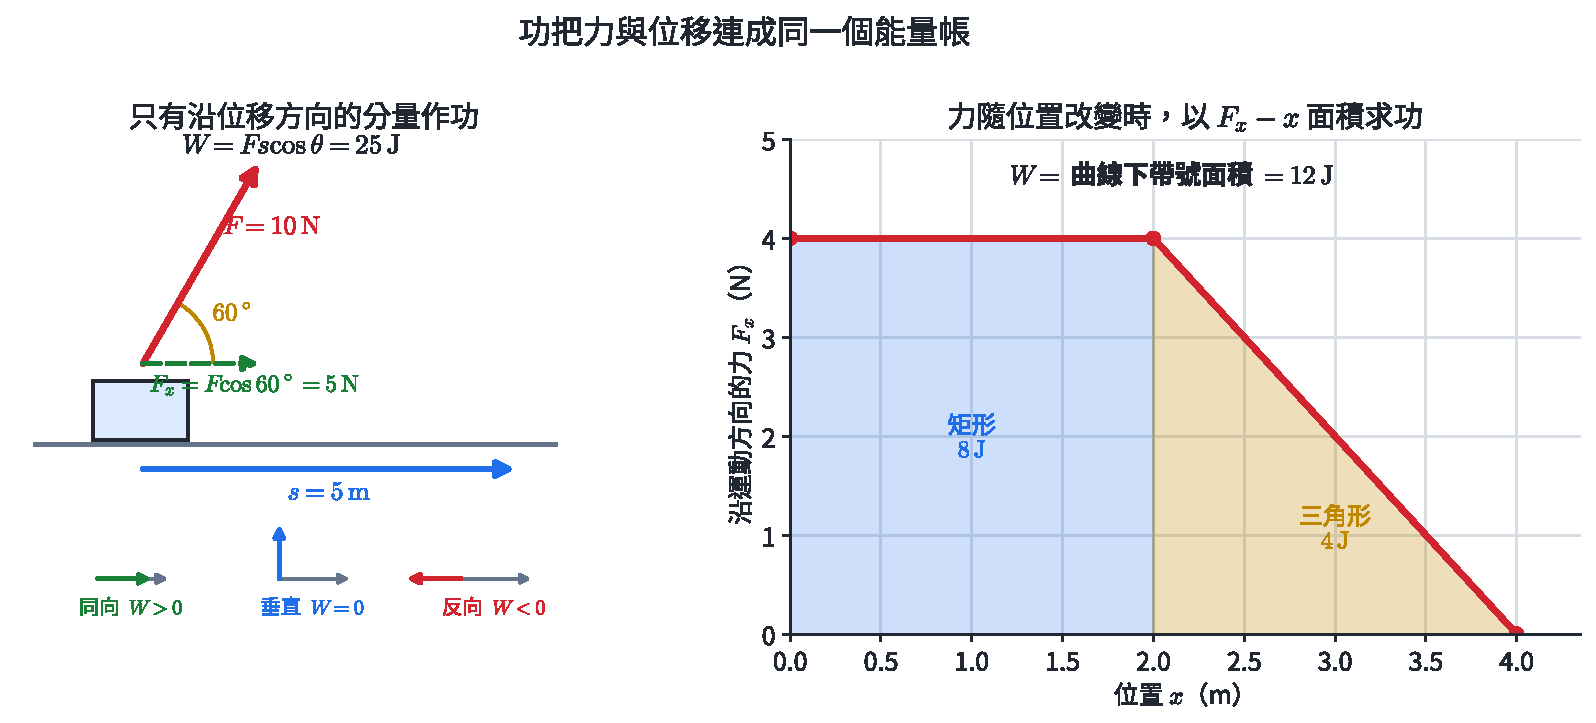
\includegraphics[keepaspectratio,alt={常力方向決定功的正負；變力功由力---位置圖的帶號面積求得}]{assets/必物-5-功的方向與力位移面積.pdf}}
\caption{常力方向決定功的正負；變力功由力---位置圖的帶號面積求得}
\end{figure}

物體受到恆力 \(\vec F\)，位移為 \(\vec s\)，兩向量夾角為 \(\theta\)。把力分解成沿位移與垂直位移的分量：

\[
F_\parallel=F\cos\theta,
\qquad
F_\perp=F\sin\theta.
\]

垂直位移的分量沒有沿該方向的位移，常力所作的功為

\[
W=F_\parallel s=Fs\cos\theta=\vec F\cdot\vec s.
\]

\begin{itemize}
\tightlist
\item
  \(0^\circ\leq\theta<90^\circ\)：\(W>0\)，該力向系統輸入機械能。
\item
  \(\theta=90^\circ\)：\(W=0\)，例如等速率圓周運動的向心力。
\item
  \(90^\circ<\theta\leq180^\circ\)：\(W<0\)，該力使物體的動能傾向減少。
\end{itemize}

功的正負屬於「某一個力」與「這段位移」的關係。同一段運動中，重力、支持力、拉力與摩擦力可各自作正功、負功或零功。

力隨位置改變時，把路徑切成許多小段，每小段近似有 \(\Delta W=F_x\Delta x\)。相加後得到

\[
W=\int_{x_i}^{x_f}F_x(x)\,dx,
\]

其幾何意義是 \(F_x-x\) 圖中曲線與橫軸之間的帶號面積。橫軸上方為正，橫軸下方為負。

\subsubsection{示範 1　斜向拉行李箱}\label{ux793aux7bc4-1-ux659cux5411ux62c9ux884cux674eux7bb1}

質量 \(20\ \mathrm{kg}\) 的行李箱在水平地面向右移動 \(6.0\ \mathrm m\)。拉力大小 \(50\ \mathrm N\)，與水平夾 \(37^\circ\)；動摩擦力為 \(24\ \mathrm N\)。取 \(\cos37^\circ=0.80\)。

\begin{enumerate}
\def\labelenumi{\arabic{enumi}.}
\item
  圖中的位移向右，拉力沿位移分量為 \(50\times0.80=40\ \mathrm N\)。
\item
  拉力作功

  \[W_F=50(6.0)\cos37^\circ=240\ \mathrm J.\]
\item
  摩擦力與位移反向：

  \[W_f=-24(6.0)=-144\ \mathrm J.\]
\item
  重力與支持力都垂直水平位移，兩者作功皆為 \(0\)。
\item
  合功為 \(W_{\mathrm{net}}=240-144=96\ \mathrm J\)。
\end{enumerate}

\subsubsection{示範 2　由力---位置圖求功}\label{ux793aux7bc4-2-ux7531ux529bux4f4dux7f6eux5716ux6c42ux529f}

物體從 \(x=0\) 移到 \(x=4.0\ \mathrm m\)。\(0\) 到 \(2.0\ \mathrm m\) 間 \(F_x=4.0\ \mathrm N\)；其後力線性降至 \(0\)。

矩形面積為 \(4.0\times2.0=8.0\ \mathrm J\)，三角形面積為 \(\frac12(2.0)(4.0)=4.0\ \mathrm J\)，所以

\[
W=8.0+4.0=12\ \mathrm J.
\]

\subsection{1.2 動能與功---動能定理}\label{ux52d5ux80fdux8207ux529fux52d5ux80fdux5b9aux7406}

質量 \(m\)、速率 \(v\) 的物體具有動能

\[
K=\frac12mv^2.
\]

動能取決於速率，方向改變而速率不變時，動能不變。速率加倍時，動能成為四倍。

沿直線運動且合力固定時，\(\sum F=ma\)。利用運動學關係 \(v_f^2-v_i^2=2as\)：

\[
W_{\mathrm{net}}=(\sum F)s=mas
=\frac12m(v_f^2-v_i^2)
=K_f-K_i.
\]

因此一般情況仍可寫成

\[
\boxed{W_{\mathrm{net}}=\Delta K}.
\]

功---動能定理直接連接「一段路徑上所有力的合功」與「初末速率」，適合分析煞車、推車、碰撞前後加速與變力問題。

\subsubsection{示範 3　煞車所需的平均力}\label{ux793aux7bc4-3-ux715eux8ecaux6240ux9700ux7684ux5e73ux5747ux529b}

質量 \(1000\ \mathrm{kg}\) 的汽車由 \(20\ \mathrm{m/s}\) 煞停，煞車距離為 \(50\ \mathrm m\)，路面對車的平均水平合力與位移反向。

\[
W_{\mathrm{net}}=\Delta K=0-\frac12(1000)(20)^2=-2.0\times10^5\ \mathrm J.
\]

若以平均力表示：

\[
-F_{\mathrm{avg}}(50)=-2.0\times10^5,
\qquad
F_{\mathrm{avg}}=4.0\times10^3\ \mathrm N.
\]

速率若增為兩倍且平均煞車力相同，初動能成為四倍，煞車距離也成為四倍。

\subsection{1.3 重力位能、彈性位能與機械能}\label{ux91cdux529bux4f4dux80fdux5f48ux6027ux4f4dux80fdux8207ux6a5fux68b0ux80fd}

\begin{figure}
\centering
\pandocbounded{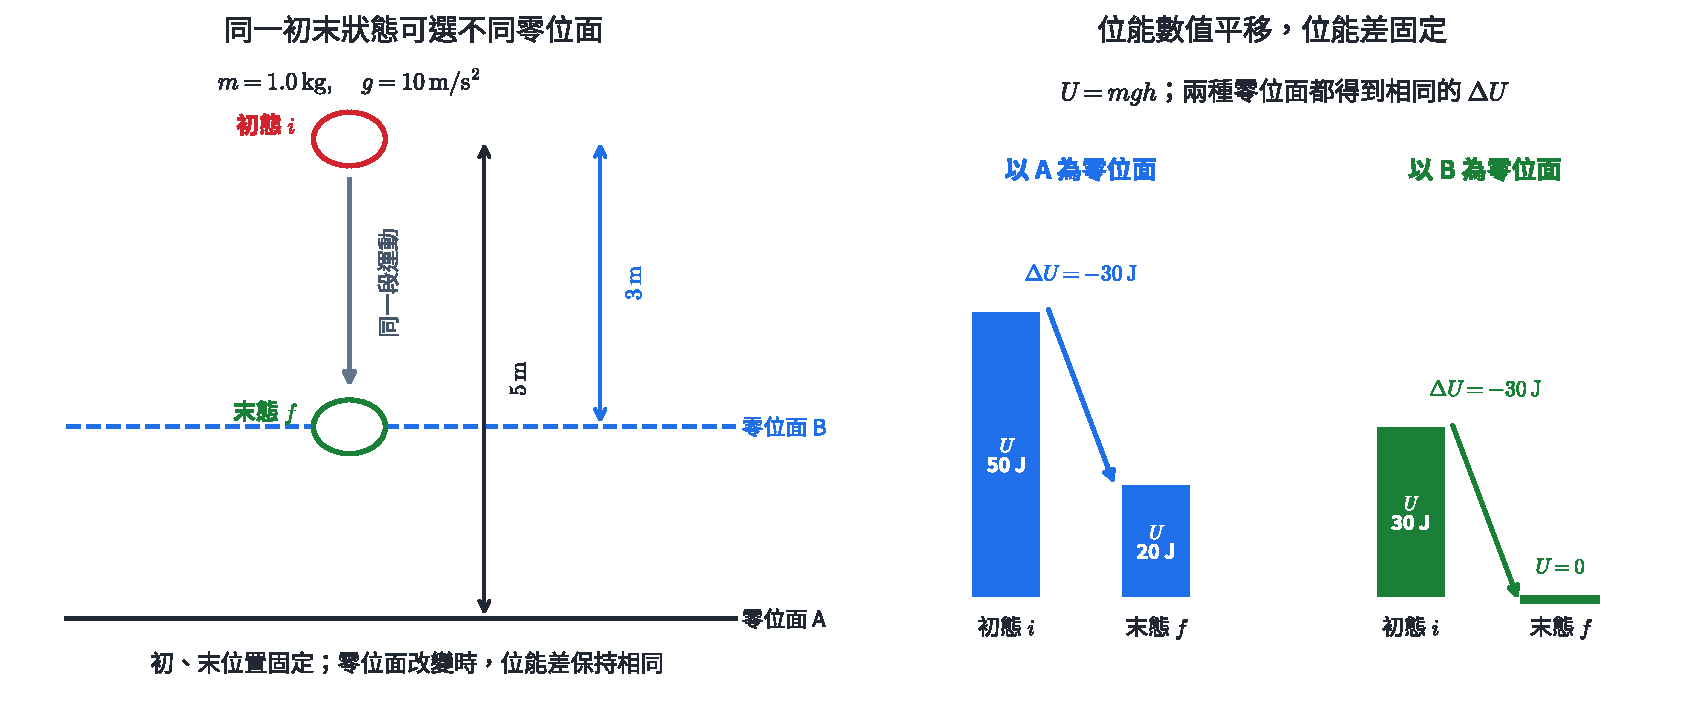
\includegraphics[keepaspectratio,alt={固定同一初末狀態，改用兩個零位面計算重力位能，兩者都得到相同位能差}]{assets/必物-5-動能位能與零位面.pdf}}
\caption{固定同一初末狀態，改用兩個零位面計算重力位能，兩者都得到相同位能差}
\end{figure}

近地面重力大小近似固定。把物體與地球合併成系統，選定高度 \(h=0\) 的零位面，重力位能定義為

\[
U_g=mgh.
\]

物體從 \(h_i\) 移到 \(h_f\) 時，重力作功為

\[
W_g=mg(h_i-h_f)=-\Delta U_g.
\]

零位面可依題目選擇。零位面改變會讓每一狀態的 \(U_g\) 同加一個常數，位能差 \(\Delta U_g\) 與可求得的速度保持相同。

彈簧在彈性限度內符合胡克定律 \(F=-kx\)。由力---位置面積可得彈性位能

\[
U_s=\frac12kx^2,
\]

其中 \(x\) 是相對平衡位置的伸長或壓縮量。物體的動能與系統的位能合稱機械能：

\[
E_{\mathrm{mech}}=K+U_g+U_s.
\]

\subsubsection{示範 4　零位面的選擇}\label{ux793aux7bc4-4-ux96f6ux4f4dux9762ux7684ux9078ux64c7}

質量 \(2.0\ \mathrm{kg}\) 的物體從地面上方 \(8.0\ \mathrm m\) 降到 \(3.0\ \mathrm m\)，取 \(g=10\ \mathrm{m/s^2}\)。

以地面為零位面：\(U_i=160\ \mathrm J\)，\(U_f=60\ \mathrm J\)。重力位能變化為

\[
\Delta U_g=60-160=-100\ \mathrm J.
\]

若改以 \(3.0\ \mathrm m\) 高度為零位面，\(U_i=100\ \mathrm J\)、\(U_f=0\)，仍有 \(\Delta U_g=-100\ \mathrm J\)；重力作功為 \(+100\ \mathrm J\)。

\subsection{1.4 功率、電能度數與效率}\label{ux529fux7387ux96fbux80fdux5ea6ux6578ux8207ux6548ux7387}

\begin{figure}
\centering
\pandocbounded{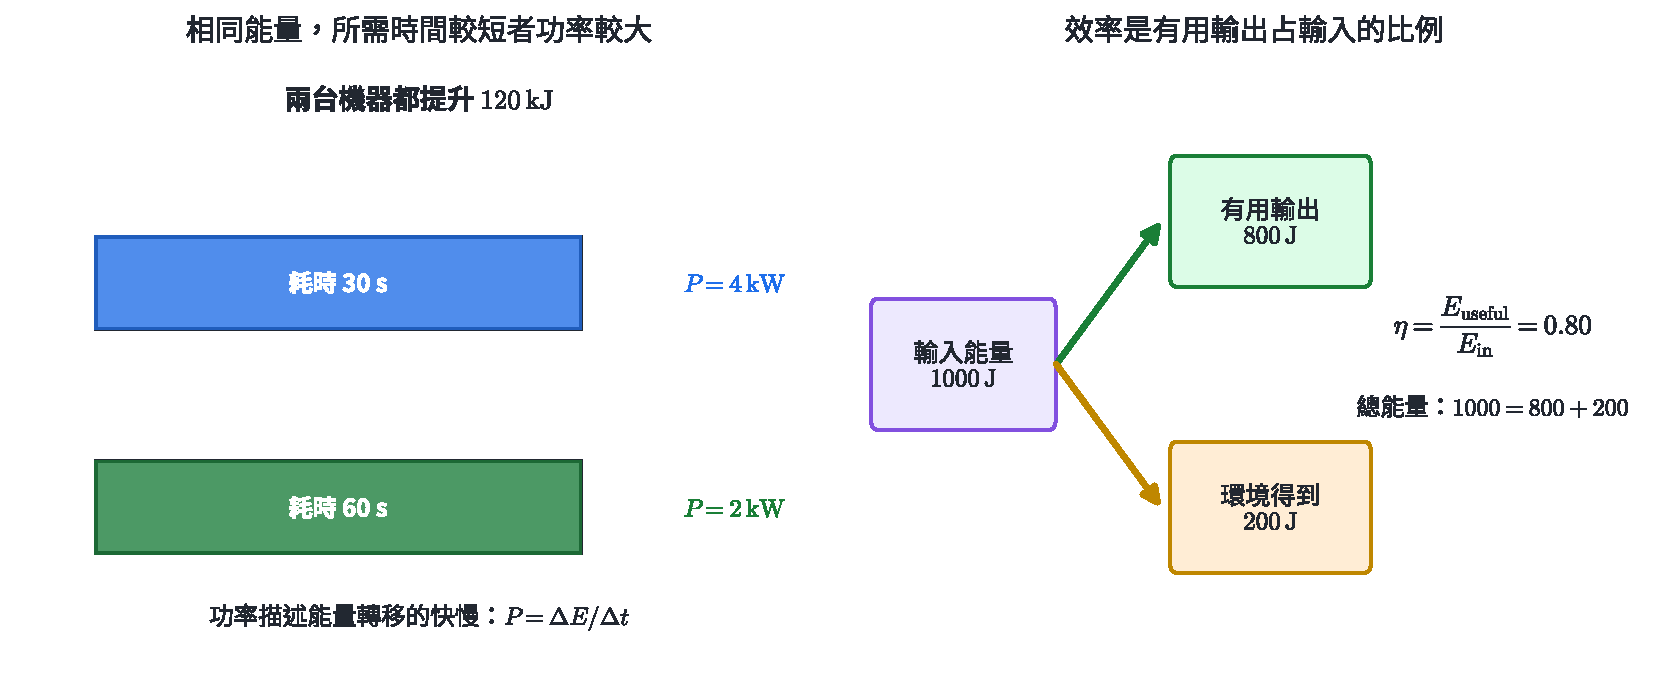
\includegraphics[keepaspectratio,alt={功率與效率能流}]{assets/必物-5-功率與效率能流.pdf}}
\caption{功率與效率能流}
\end{figure}

平均功率是能量轉移量除以所需時間：

\[
P_{\mathrm{avg}}=\frac{W}{\Delta t}=\frac{\Delta E}{\Delta t}.
\]

恆力與速度同方向時，\(W=Fs\) 且 \(s=v\Delta t\)，所以瞬時功率可寫成 \(P=Fv\)；一般向量式為 \(P=\vec F\cdot\vec v\)。

電費常用千瓦小時（kWh）作為能量單位：

\[
1\ \mathrm{kWh}=(1000\ \mathrm W)(3600\ \mathrm s)
=3.6\times10^6\ \mathrm J.
\]

裝置的效率為

\[
\eta=\frac{E_{\mathrm{useful}}}{E_{\mathrm{in}}}
=\frac{P_{\mathrm{useful}}}{P_{\mathrm{in}}}.
\]

有用輸出的判定取決於任務。燈具的有用輸出是照明所需的可見光；熱水器的有用輸出是水增加的內能。其餘能量仍流向裝置或環境。

\subsubsection{示範 5　抽水馬達}\label{ux793aux7bc4-5-ux62bdux6c34ux99acux9054}

馬達在 \(25\ \mathrm s\) 內把 \(200\ \mathrm{kg}\) 的水提升 \(15\ \mathrm m\)，取 \(g=10\ \mathrm{m/s^2}\)。輸入電功率為 \(1.5\ \mathrm{kW}\)。

水增加的重力位能：

\[
\Delta U_g=mgh=(200)(10)(15)=3.0\times10^4\ \mathrm J.
\]

有用輸出功率為 \(3.0\times10^4/25=1.2\times10^3\ \mathrm W\)，效率

\[
\eta=\frac{1.2\ \mathrm{kW}}{1.5\ \mathrm{kW}}=0.80=80\%.
\]

\subsection{本節練習}\label{ux672cux7bc0ux7df4ux7fd2}

\begin{enumerate}
\def\labelenumi{\arabic{enumi}.}
\tightlist
\item
  水平推力 \(30\ \mathrm N\) 使箱子向右移動 \(4.0\ \mathrm m\)，推力作功多少？
\item
  人以 \(80\ \mathrm N\) 的力提著書包等速水平前進 \(10\ \mathrm m\)，提力對書包作功多少？
\item
  \(F_x-x\) 圖在 \(0\) 至 \(3.0\ \mathrm m\) 為 \(+6.0\ \mathrm N\)，在 \(3.0\) 至 \(5.0\ \mathrm m\) 為 \(-2.0\ \mathrm N\)。總功多少？
\item
  \(2.0\ \mathrm{kg}\) 物體速率由 \(3.0\ \mathrm{m/s}\) 增至 \(7.0\ \mathrm{m/s}\)，合功多少？
\item
  \(0.50\ \mathrm{kg}\) 球位於零位面上方 \(12\ \mathrm m\)，取 \(g=10\ \mathrm{m/s^2}\)。其重力位能多少？若零位面上移 \(2.0\ \mathrm m\)，位能改為多少？
\item
  \(1200\ \mathrm W\) 電器運作 \(15\ \mathrm{min}\)，耗能多少 J、多少 kWh？
\end{enumerate}

答案：1. \(120\ \mathrm J\)。2. \(0\)。3. \(14\ \mathrm J\)。4. \(40\ \mathrm J\)。5. \(60\ \mathrm J\)；\(50\ \mathrm J\)。6. \(1.08\times10^6\ \mathrm J=0.30\ \mathrm{kWh}\)。

\section{2　微觀尺度下的能量}\label{ux5faeux89c0ux5c3aux5ea6ux4e0bux7684ux80fdux91cf}

\subsection{2.1 理想氣體模型、溫度與內能}\label{ux7406ux60f3ux6c23ux9ad4ux6a21ux578bux6eabux5ea6ux8207ux5167ux80fd}

\begin{figure}
\centering
\pandocbounded{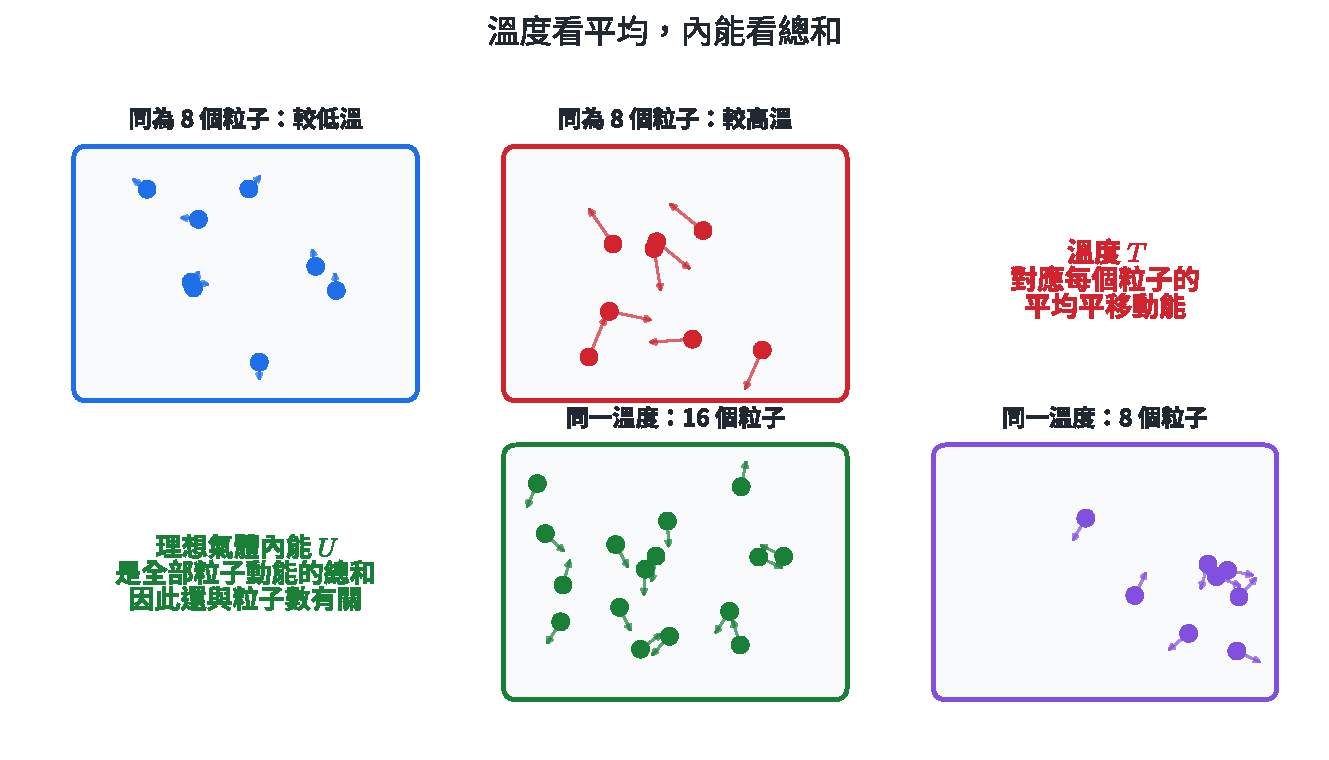
\includegraphics[keepaspectratio,alt={溫度、內能與粒子數}]{assets/必物-5-溫度內能與粒子數.pdf}}
\caption{溫度、內能與粒子數}
\end{figure}

理想氣體模型把氣體描述成大量持續無規則運動的粒子，採用下列條件：

\begin{enumerate}
\def\labelenumi{\arabic{enumi}.}
\tightlist
\item
  粒子本身體積相對容器可忽略。
\item
  除碰撞瞬間外，粒子間作用力可忽略。
\item
  粒子彼此及與容器壁的碰撞為彈性碰撞。
\item
  粒子運動方向無規則，宏觀壓力來自粒子撞擊器壁。
\end{enumerate}

溫度反映粒子無規則運動的平均動能。理想氣體的內能是所有粒子動能的總和，因此同溫度、粒子數較多的樣品具有較多內能。真實氣體還可能包含分子間位能，尤其在高壓或接近液化時，理想氣體近似的誤差會增大。

{\def\LTcaptype{none} % do not increment counter
\begin{longtable}[]{@{}ll@{}}
\toprule\noalign{}
比較 & 微觀判讀 \\
\midrule\noalign{}
\endhead
\bottomrule\noalign{}
\endlastfoot
同一種氣體、同粒子數，溫度較高 & 平均分子動能較大，內能較大 \\
同一種氣體、同溫度，粒子數較多 & 平均分子動能相同，總內能較大 \\
同一杯水達熱平衡 & 分子仍持續運動，宏觀溫度保持穩定 \\
\end{longtable}
}

布朗運動是懸浮微粒受到周圍分子不均勻碰撞而呈現的曲折運動。可見微粒的軌跡提供分子持續運動的間接證據。

\subsubsection{示範 6　平均與總和}\label{ux793aux7bc4-6-ux5e73ux5747ux8207ux7e3dux548c}

A、B 兩個容器裝同種理想氣體。A 有 \(N\) 個粒子、溫度 \(300\ \mathrm K\)；B 有 \(2N\) 個粒子、溫度也為 \(300\ \mathrm K\)。

\begin{itemize}
\tightlist
\item
  兩容器每粒子的平均動能相同。
\item
  B 的粒子數是 A 的兩倍，所以 B 的總內能是 A 的兩倍。
\end{itemize}

若 A 升到 \(600\ \mathrm K\) 而粒子數不變，A 的平均動能與內能都變為原來兩倍。

\subsection{2.2 熱與熱平衡}\label{ux71b1ux8207ux71b1ux5e73ux8861}

熱是因溫度差而在系統間傳遞的能量。兩物體接觸時，淨能量由高溫物體流向低溫物體；達到相同溫度後稱為熱平衡，巨觀上不再有淨熱傳。

物體的內能可以藉由兩種途徑改變：外界對系統作功，或系統與外界因溫差交換熱。例如壓縮氣體、摩擦與攪拌可藉作功增加內能；加熱器則以能量傳遞使水的內能增加。

微波爐中的交變電場促使極性水分子反覆轉向，分子碰撞使無規則運動能量增加。食物中含水量與形狀不同，吸收與散熱條件也不同，因此加熱可能不均勻。

\subsubsection{示範 7　兩杯水混合的方向判斷}\label{ux793aux7bc4-7-ux5169ux676fux6c34ux6df7ux5408ux7684ux65b9ux5411ux5224ux65b7}

絕熱容器中有 \(200\ \mathrm g\)、\(80^\circ\mathrm C\) 的水與 \(200\ \mathrm g\)、\(20^\circ\mathrm C\) 的水。兩者比熱相同且容器吸熱忽略。

高溫水失去的能量等於低溫水得到的能量：

\[
mc(80-T_f)=mc(T_f-20).
\]

約去相同的 \(mc\)，得 \(T_f=50^\circ\mathrm C\)。末溫介於兩個初溫之間，符合能量由高溫端流向低溫端的判讀。

\subsection{2.3 絕對溫標}\label{ux7d55ux5c0dux6eabux6a19}

\begin{figure}
\centering
\pandocbounded{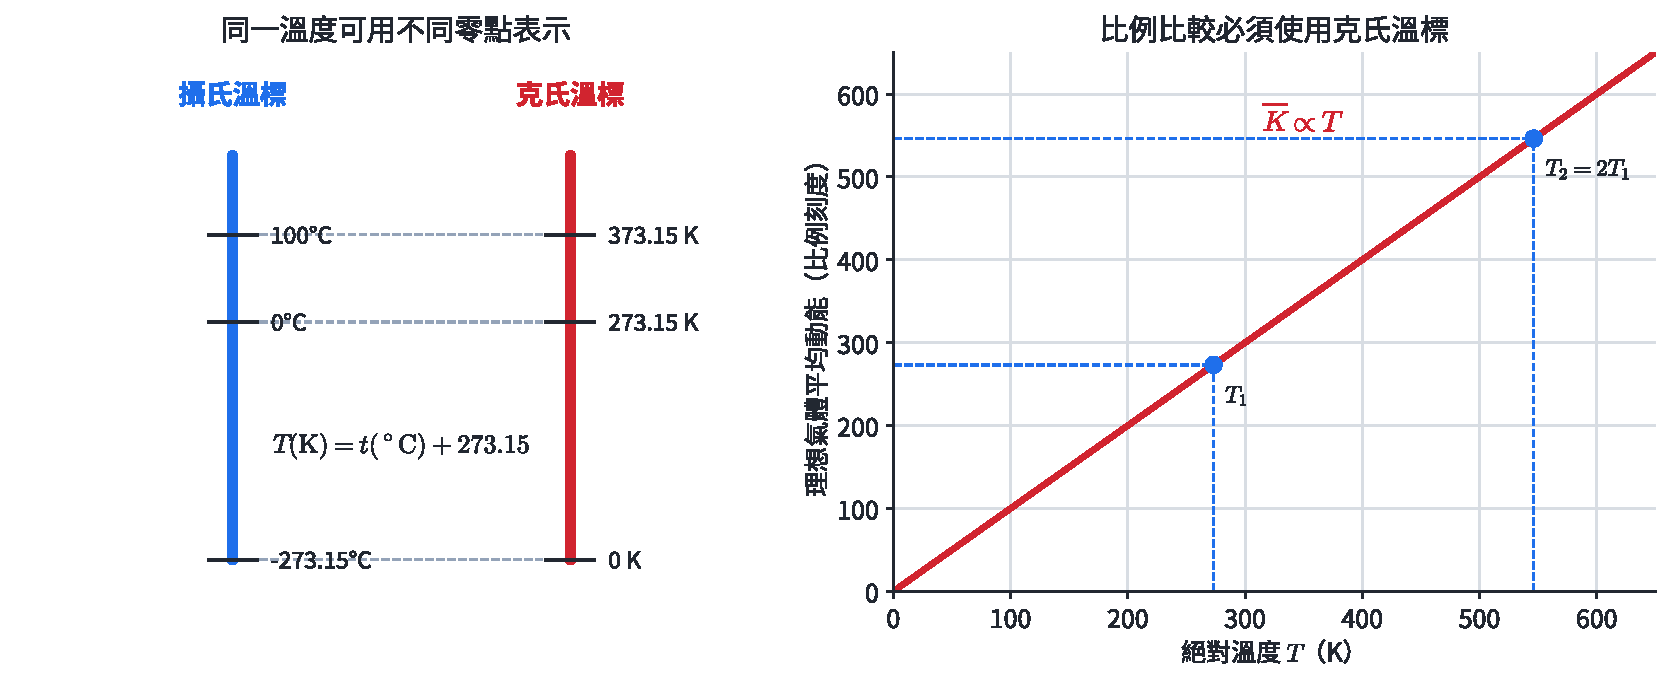
\includegraphics[keepaspectratio,alt={攝氏、克氏與平均動能}]{assets/必物-5-攝氏克氏與平均動能.pdf}}
\caption{攝氏、克氏與平均動能}
\end{figure}

攝氏溫標與克氏溫標每一度的大小相同，零點不同：

\[
T(\mathrm K)=t(^\circ\mathrm C)+273.15.
\]

\(0\ \mathrm K\) 稱為絕對零度，是古典理想氣體模型中平均平移動能趨近最低的理論界線。理想氣體分子的平均平移動能與絕對溫度成正比，因此溫度倍數必須用 K 比較。

\subsubsection{示範 8　攝氏差值與克氏倍數}\label{ux793aux7bc4-8-ux651dux6c0fux5deeux503cux8207ux514bux6c0fux500dux6578}

氣體由 \(27^\circ\mathrm C\) 升到 \(327^\circ\mathrm C\)。兩個溫度分別約為 \(300\ \mathrm K\) 與 \(600\ \mathrm K\)，所以平均分子動能成為兩倍。攝氏讀數由 27 變成 327，直接以 \(327/27\) 比較沒有絕對溫度的物理意義。

\subsection{本節練習}\label{ux672cux7bc0ux7df4ux7fd2-1}

\begin{enumerate}
\def\labelenumi{\arabic{enumi}.}
\tightlist
\item
  同種理想氣體的兩個樣品，A 有 \(N\) 個粒子、B 有 \(3N\) 個粒子，兩者同溫。比較平均分子動能與總內能。
\item
  將 \(25^\circ\mathrm C\)、\(-40^\circ\mathrm C\) 分別換算成 K。
\item
  理想氣體由 \(250\ \mathrm K\) 升至 \(500\ \mathrm K\)，平均分子動能成為幾倍？
\item
  同質量、同材質的金屬塊分別為 \(80^\circ\mathrm C\) 與 \(20^\circ\mathrm C\)，接觸且與外界絕熱。熱的淨傳遞方向為何？達平衡後兩塊內部粒子是否停止運動？
\item
  A 杯有 \(100\ \mathrm g\)、\(60^\circ\mathrm C\) 的水；B 杯有 \(300\ \mathrm g\)、\(60^\circ\mathrm C\) 的水。比較溫度、平均分子動能與總內能。
\item
  說明布朗運動中顯微鏡下可見微粒的曲折軌跡所提供的證據。
\end{enumerate}

答案：1. 平均動能相同；B 的總內能為 A 的三倍。2. \(298.15\ \mathrm K\)；\(233.15\ \mathrm K\)。3. 兩倍。4. 由 \(80^\circ\mathrm C\) 物體流向 \(20^\circ\mathrm C\) 物體；粒子仍持續運動。5. 溫度與平均動能相同；B 的總內能較大，在理想化同狀態近似下約為三倍。6. 周圍分子持續無規則運動並以不均勻碰撞推動微粒。

\section{3　能量守恆與能量轉換}\label{ux80fdux91cfux5b88ux6046ux8207ux80fdux91cfux8f49ux63db}

\subsection{3.1 先指定系統，再寫能量帳}\label{ux5148ux6307ux5b9aux7cfbux7d71ux518dux5bebux80fdux91cfux5e33}

能量守恆指封閉系統的總能量保持不變。分析實際問題時，先畫出系統邊界，再把跨越邊界的能量列入：

\[
\boxed{E_i+E_{\mathrm{in}}=E_f+E_{\mathrm{out}}}.
\]

\(E_i\)、\(E_f\) 是系統初、末儲存的能量；\(E_{\mathrm{in}}\)、\(E_{\mathrm{out}}\) 是藉作功、電流、熱傳或輻射跨越邊界的能量。同一現象採用不同系統，帳的寫法會改變，最後可觀測結果必須一致。

例如把「球」當系統，下降時重力是外力，重力對球作正功；把「球＋地球」當系統，重力作用位於系統內部，帳上呈現為重力位能轉為動能。

\subsection{3.2 力學能守恆}\label{ux529bux5b78ux80fdux5b88ux6046}

\begin{figure}
\centering
\pandocbounded{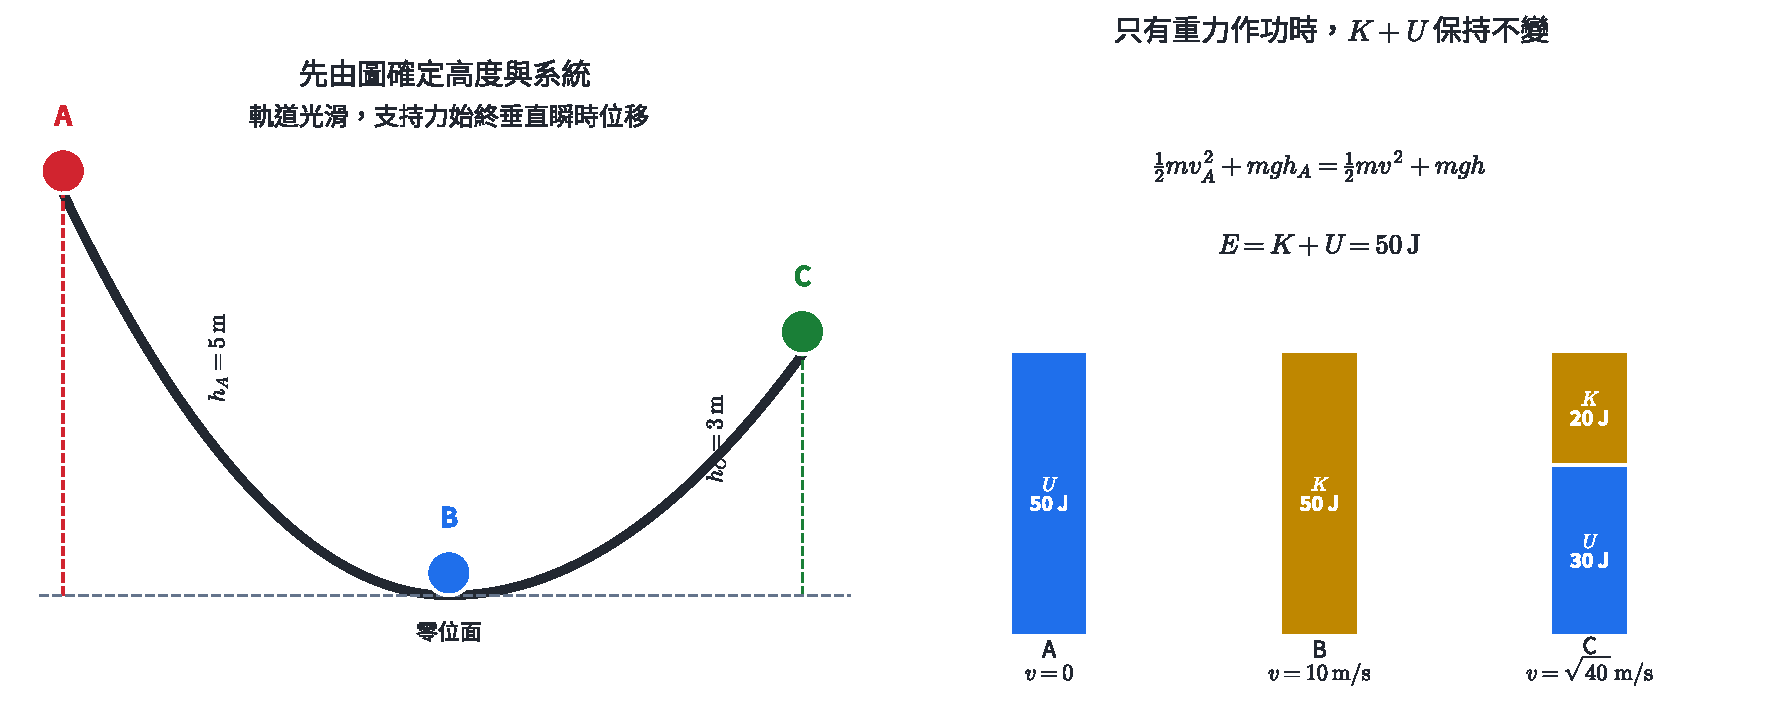
\includegraphics[keepaspectratio,alt={光滑軌道上的力學能守恆}]{assets/必物-5-軌道力學能守恆.pdf}}
\caption{光滑軌道上的力學能守恆}
\end{figure}

對物體使用功---動能定理：

\[
\Delta K=W_g+W_{\mathrm{other}}.
\]

重力作功 \(W_g=-\Delta U_g\)，代入後得到

\[
\Delta K+\Delta U_g=W_{\mathrm{other}}.
\]

當其他力的總功為零，例如光滑固定軌道的支持力始終垂直位移，便有

\[
\boxed{K_i+U_i=K_f+U_f}.
\]

若系統也含理想彈簧，則把 \(U_s\) 加入。力學能守恆的條件可表述為：系統內只有重力、理想彈力等保守作用在動能與位能間轉換；跨系統邊界的外力作功為零，且沒有摩擦造成的熱能增加。

\subsubsection{示範 9　滑板通過光滑 U 形軌道}\label{ux793aux7bc4-9-ux6ed1ux677fux901aux904eux5149ux6ed1-u-ux5f62ux8eccux9053}

質量 \(1.0\ \mathrm{kg}\) 的滑板由 A 點靜止下滑，A 比最低點 B 高 \(5.0\ \mathrm m\)，C 比 B 高 \(3.0\ \mathrm m\)。軌道光滑，取 \(g=10\ \mathrm{m/s^2}\)。

選滑板與地球為系統，以 B 為重力位能零位面。

在 B 點：

\[
mgh_A=\frac12mv_B^2,
\qquad
v_B=\sqrt{2gh_A}=10\ \mathrm{m/s}.
\]

在 C 點：

\[
mgh_A=\frac12mv_C^2+mgh_C,
\]

\[
v_C=\sqrt{2g(h_A-h_C)}=\sqrt{40}\approx6.3\ \mathrm{m/s}.
\]

質量在方程兩側約去，表示相同初始高度與相同軌道條件下，理想模型預測速度與質量無關。

\subsubsection{示範 10　外力提升物體}\label{ux793aux7bc4-10-ux5916ux529bux63d0ux5347ux7269ux9ad4}

起重機使 \(500\ \mathrm{kg}\) 貨物由靜止開始，上升 \(8.0\ \mathrm m\) 後速率為 \(4.0\ \mathrm{m/s}\)。取 \(g=10\ \mathrm{m/s^2}\)，忽略阻力。

貨物與地球系統的機械能增加量為

\[
\Delta E_{\mathrm{mech}}=\Delta K+\Delta U_g
=\frac12(500)(4.0)^2+(500)(10)(8.0)
=4.4\times10^4\ \mathrm J.
\]

這個能量由起重機對系統作功輸入，所以起重機作功 \(4.4\times10^4\ \mathrm J\)。

\subsection{3.3 摩擦下的總能量守恆}\label{ux6469ux64e6ux4e0bux7684ux7e3dux80fdux91cfux5b88ux6046}

\begin{figure}
\centering
\pandocbounded{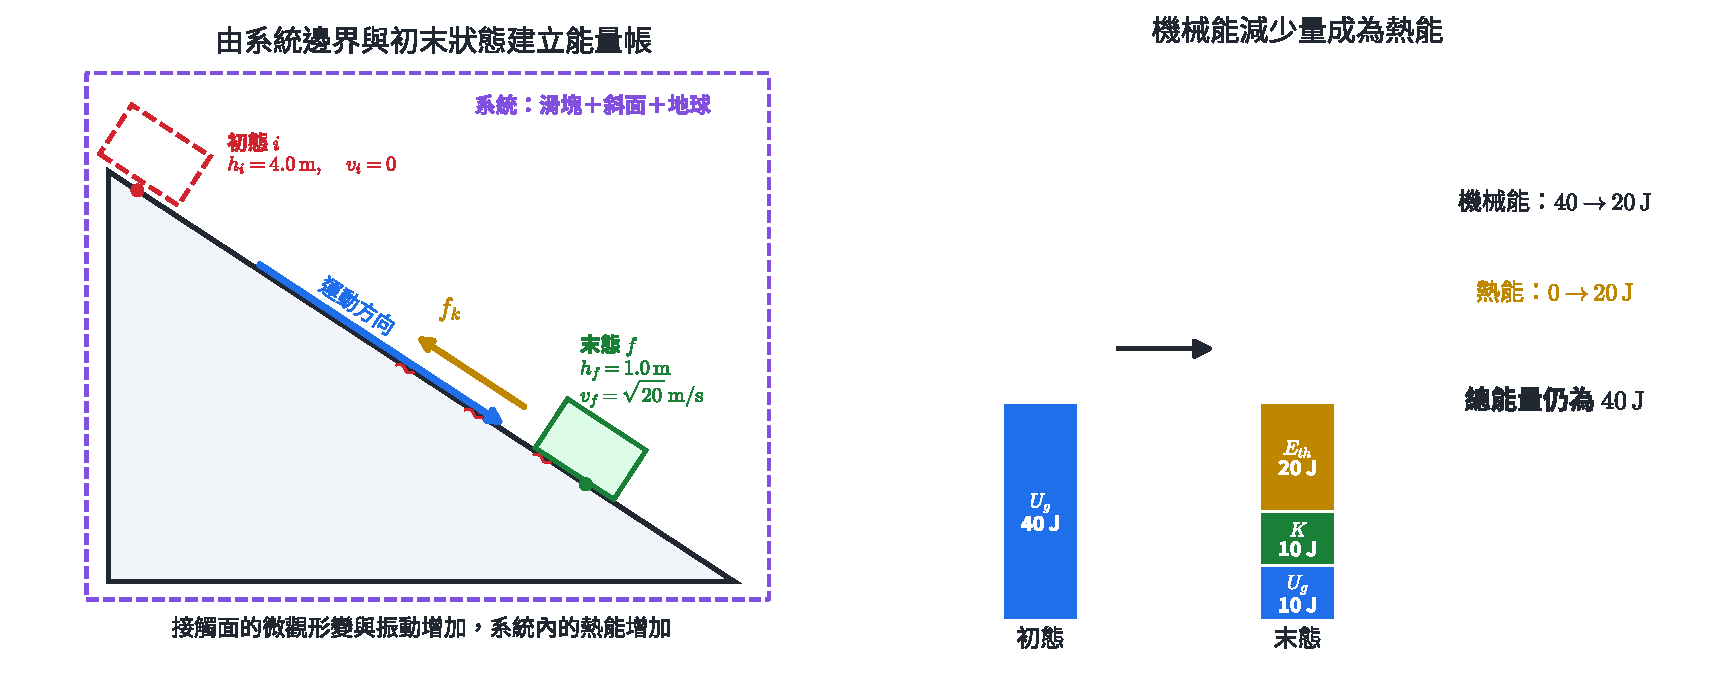
\includegraphics[keepaspectratio,alt={滑塊、斜面與地球位於同一系統邊界內；初末狀態的機械能差轉為系統熱能}]{assets/必物-5-摩擦下的能量帳.pdf}}
\caption{滑塊、斜面與地球位於同一系統邊界內；初末狀態的機械能差轉為系統熱能}
\end{figure}

摩擦使接觸面的微觀形變與無規則振動增加，宏觀上表現為熱能增加。若物體與接觸面都包含在系統內，且與外界沒有能量交換：

\[
K_i+U_i+E_{{\mathrm{th}},i}
=K_f+U_f+E_{{\mathrm{th}},f}.
\]

熱能增加量等於機械能減少量：

\[
\Delta E_{\mathrm{th}}=-(\Delta K+\Delta U).
\]

總能量守恆並保留各種形式的總量；能量轉成大量粒子的無規則運動後，能夠整體轉回宏觀作功的比例通常降低。煞車碟升溫、輪胎與路面升溫、空氣擾動與聲音都可列入能量去向。

\subsubsection{示範 11　粗糙斜面上的滑塊}\label{ux793aux7bc4-11-ux7c97ux7cd9ux659cux9762ux4e0aux7684ux6ed1ux584a}

\(2.0\ \mathrm{kg}\) 滑塊由靜止從高 \(4.0\ \mathrm m\) 處滑下，到達高 \(1.0\ \mathrm m\) 處時速率為 \(4.0\ \mathrm{m/s}\)。取 \(g=10\ \mathrm{m/s^2}\)。

初機械能為 \(E_i=(2)(10)(4)=80\ \mathrm J\)。末機械能為

\[
E_f=\frac12(2)(4)^2+(2)(10)(1)=16+20=36\ \mathrm J.
\]

因此物體與斜面增加的熱能為

\[
\Delta E_{\mathrm{th}}=80-36=44\ \mathrm J.
\]

\subsection{3.4 作功、熱與內能}\label{ux4f5cux529fux71b1ux8207ux5167ux80fd}

\begin{figure}
\centering
\pandocbounded{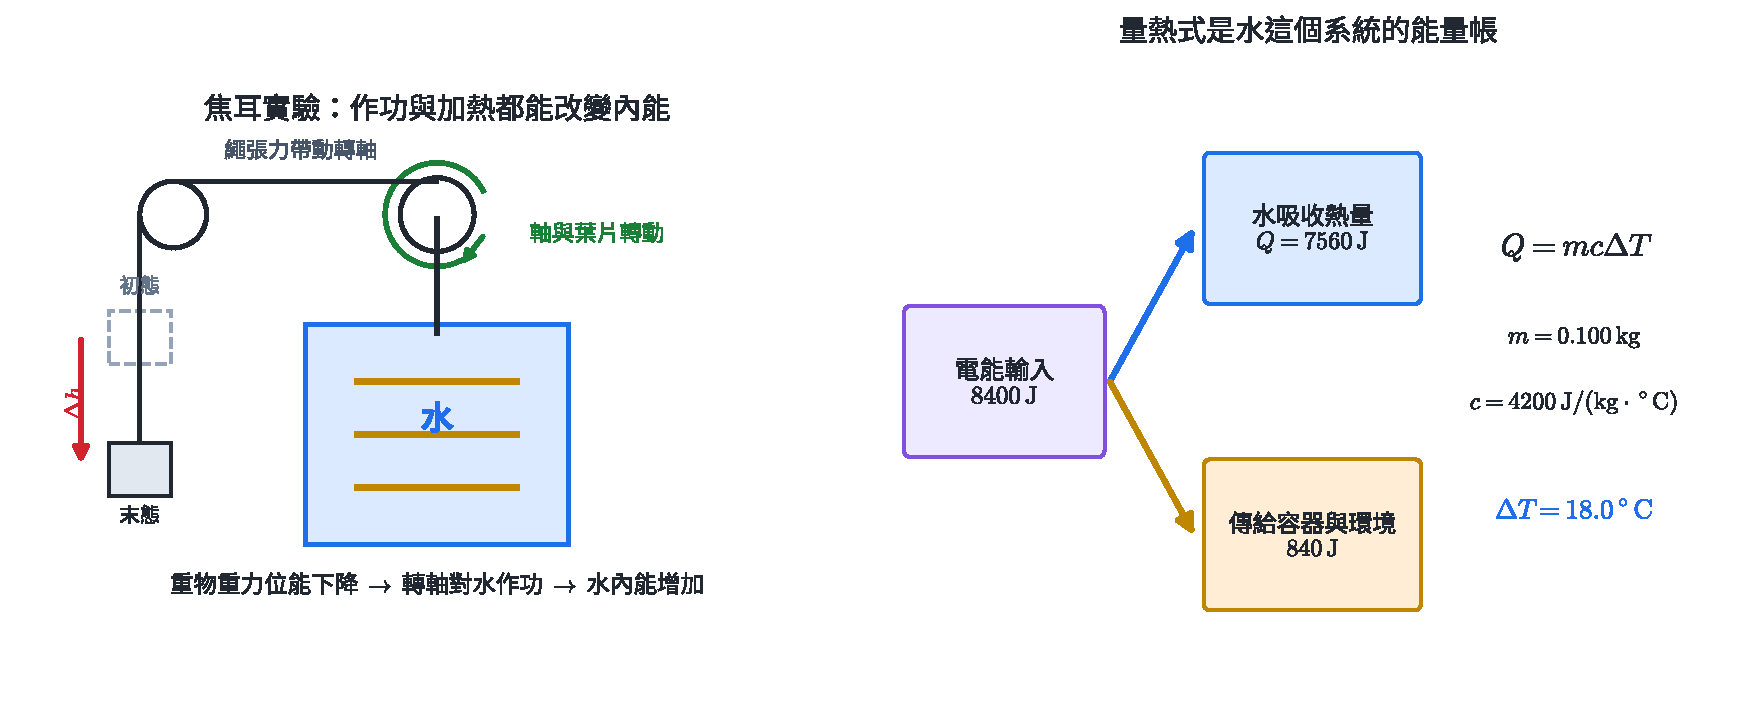
\includegraphics[keepaspectratio,alt={下降重物經滑輪帶動轉軸與水中葉片，並以能量分流計算水吸收的熱量}]{assets/必物-5-作功加熱與熱量.pdf}}
\caption{下降重物經滑輪帶動轉軸與水中葉片，並以能量分流計算水吸收的熱量}
\end{figure}

焦耳攪水實驗讓重物下降，透過滑輪帶動水中的葉片。重物減少的重力位能經葉片作功，最後成為水與容器增加的內能。實驗建立機械功與熱量可以用同一能量單位表示：

\[
1\ \mathrm{cal}\approx4.2\ \mathrm J.
\]

物質沒有發生相變、比熱可視為定值時，質量 \(m\) 的物體溫度改變 \(\Delta T\) 所交換的熱量大小為

\[
Q=mc\Delta T.
\]

此式描述特定系統吸收或放出的能量。加熱器的輸入能量還可能分給容器與環境，因而常搭配效率：

\[
\eta E_{\mathrm{electric}}=mc\Delta T.
\]

\subsubsection{示範 12　電熱器加熱水}\label{ux793aux7bc4-12-ux96fbux71b1ux5668ux52a0ux71b1ux6c34}

\(800\ \mathrm W\) 電熱器加熱 \(0.50\ \mathrm{kg}\) 的水 \(3.0\ \mathrm{min}\)，水溫由 \(20^\circ\mathrm C\) 升至 \(75^\circ\mathrm C\)。取水的比熱 \(c=4200\ \mathrm{J/(kg\cdot{}^\circ C)}\)。

輸入電能：

\[
E_{\mathrm{in}}=Pt=(800)(180)=1.44\times10^5\ \mathrm J.
\]

水吸收的能量：

\[
Q=mc\Delta T=(0.50)(4200)(55)=1.155\times10^5\ \mathrm J.
\]

效率為

\[
\eta=\frac{1.155\times10^5}{1.44\times10^5}
\approx0.802=80.2\%.
\]

其餘約 \(2.85\times10^4\ \mathrm J\) 流向容器與環境。

\subsection{3.5 能量轉換鏈與儲能}\label{ux80fdux91cfux8f49ux63dbux93c8ux8207ux5132ux80fd}

\begin{figure}
\centering
\pandocbounded{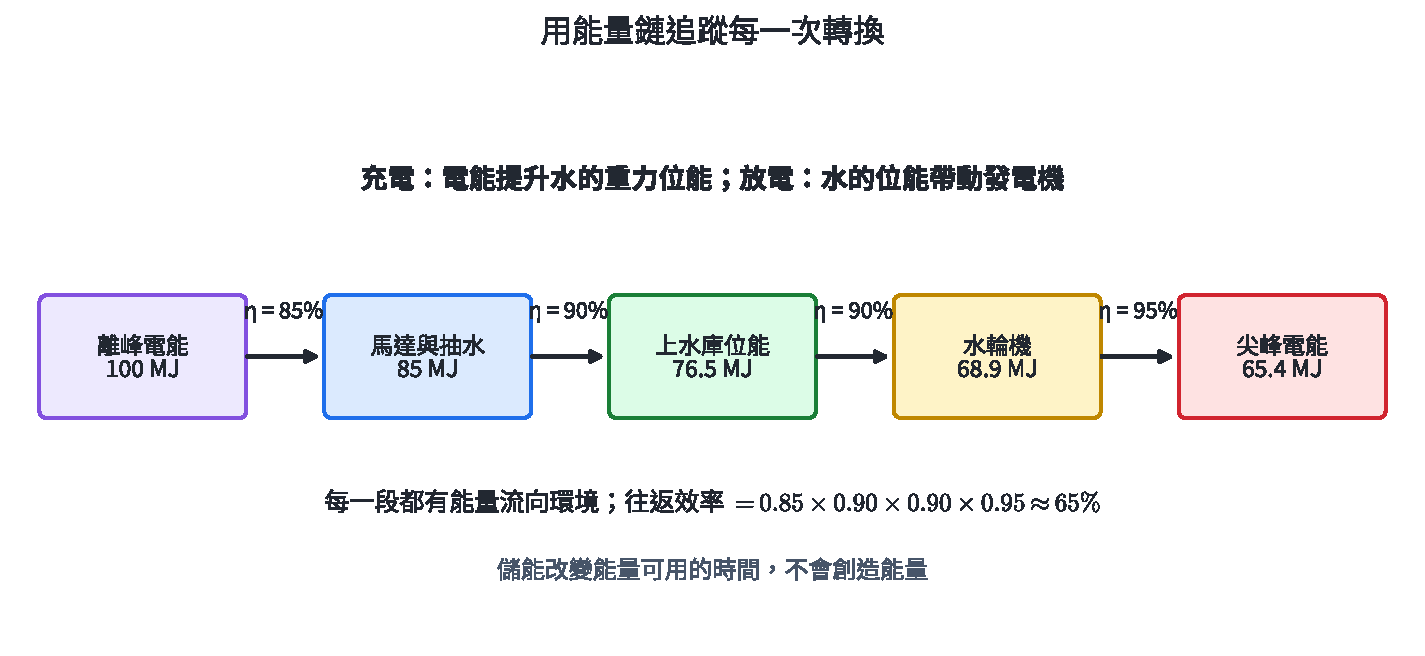
\includegraphics[keepaspectratio,alt={抽蓄發電的能量轉換鏈}]{assets/必物-5-抽蓄發電能量轉換鏈.pdf}}
\caption{抽蓄發電的能量轉換鏈}
\end{figure}

發電與用電裝置可用箭頭標示每一步能量形式：

\begin{itemize}
\tightlist
\item
  水力發電：水的重力位能 \(\rightarrow\) 水與渦輪的動能 \(\rightarrow\) 電能。
\item
  火力發電：燃料化學能 \(\rightarrow\) 內能 \(\rightarrow\) 蒸汽與渦輪動能 \(\rightarrow\) 電能。
\item
  太陽能電池：入射電磁能 \(\rightarrow\) 電能。
\item
  LED：電能 \(\rightarrow\) 可見光與熱能。
\item
  抽蓄儲能：離峰電能 \(\rightarrow\) 水的重力位能；尖峰時再反向轉換。
\end{itemize}

若各段效率分別為 \(\eta_1,\eta_2,\ldots\)，整條鏈的效率為

\[
\eta_{\mathrm{total}}=\eta_1\eta_2\cdots.
\]

\subsubsection{示範 13　多段轉換效率}\label{ux793aux7bc4-13-ux591aux6bb5ux8f49ux63dbux6548ux7387}

儲能系統充電效率為 \(85\%\)，放電端水輪機效率 \(90\%\)、發電機效率 \(95\%\)。輸入 \(200\ \mathrm{MJ}\) 電能後，可回收的電能為

\[
E_{\mathrm{out}}=(200)(0.85)(0.90)(0.95)
=145.35\ \mathrm{MJ}.
\]

往返效率為 \(72.7\%\)。儲能的功能是把可用能量移到另一時間，系統總輸出受各段效率共同限制。

\subsection{本節練習}\label{ux672cux7bc0ux7df4ux7fd2-2}

\begin{enumerate}
\def\labelenumi{\arabic{enumi}.}
\tightlist
\item
  球由靜止自 \(20\ \mathrm m\) 高處落下，忽略空氣阻力，取 \(g=10\ \mathrm{m/s^2}\)。落地前速率多少？
\item
  光滑軌道上物體在 A 點速率 \(6.0\ \mathrm{m/s}\)，移到比 A 高 \(1.0\ \mathrm m\) 的 B 點。取 \(g=10\ \mathrm{m/s^2}\)，B 點速率多少？
\item
  \(1.0\ \mathrm{kg}\) 物體由高 \(5.0\ \mathrm m\) 處靜止下滑，到底端速率 \(8.0\ \mathrm{m/s}\)。取 \(g=10\ \mathrm{m/s^2}\)，熱能增加多少？
\item
  \(0.20\ \mathrm{kg}\) 的水升溫 \(30^\circ\mathrm C\)，取 \(c=4200\ \mathrm{J/(kg\cdot{}^\circ C)}\)。水吸收多少能量？
\item
  \(1000\ \mathrm W\)、效率 \(84\%\) 的加熱器，把 \(0.50\ \mathrm{kg}\) 水升溫 \(20^\circ\mathrm C\)，至少需多少秒？
\item
  某轉換鏈三段效率依序為 \(80\%\)、\(75\%\)、\(90\%\)。輸入 \(1.0\ \mathrm{MJ}\)，有用輸出多少？總效率多少？
\end{enumerate}

答案：1. \(20\ \mathrm{m/s}\)。2. \(4.0\ \mathrm{m/s}\)。3. \(18\ \mathrm J\)。4. \(2.52\times10^4\ \mathrm J\)。5. \(50\ \mathrm s\)。6. \(5.4\times10^5\ \mathrm J\)；\(54\%\)。

\section{4　質能互換與核能}\label{ux8ceaux80fdux4e92ux63dbux8207ux6838ux80fd}

\subsection{4.1 質能關係與核反應帳}\label{ux8ceaux80fdux95dcux4fc2ux8207ux6838ux53cdux61c9ux5e33}

\begin{figure}
\centering
\pandocbounded{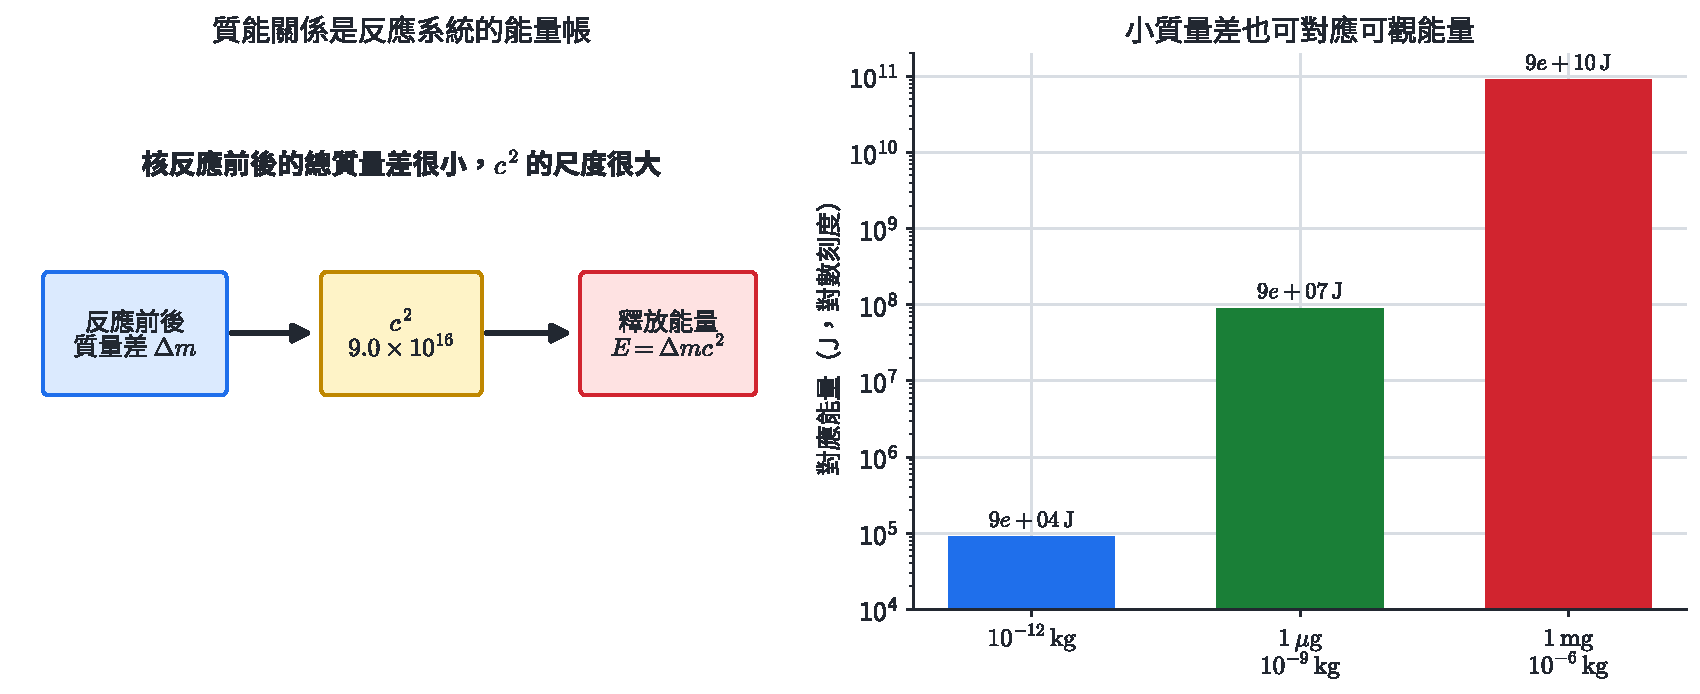
\includegraphics[keepaspectratio,alt={質量虧損與能量尺度}]{assets/必物-5-質量虧損與能量尺度.pdf}}
\caption{質量虧損與能量尺度}
\end{figure}

相對論指出，靜止質量 \(m\) 對應靜止能量 \(E_0=mc^2\)。一個封閉反應系統若反應後粒子的總靜止質量比反應前少 \(\Delta m\)，差值對應到產物動能與電磁輻射等能量：

\[
\boxed{E_{\mathrm{released}}=\Delta mc^2},
\qquad c\approx3.0\times10^8\ \mathrm{m/s}.
\]

\(c^2=9.0\times10^{16}\ \mathrm{m^2/s^2}\)，所以很小的質量差也可對應可觀能量。核反應式另須核對兩套整數帳：

\begin{enumerate}
\def\labelenumi{\arabic{enumi}.}
\tightlist
\item
  質量數 \(A\)：質子數與中子數的總和。
\item
  原子序 \(Z\)：質子數，也決定元素種類。
\end{enumerate}

反應前後 \(A\) 與 \(Z\) 各自相等；精確靜止質量可以不同，差值進入質能關係。

\subsubsection{示範 14　質量虧損所對應的能量}\label{ux793aux7bc4-14-ux8ceaux91cfux8667ux640dux6240ux5c0dux61c9ux7684ux80fdux91cf}

某反應的總質量減少 \(2.0\times10^{-11}\ \mathrm{kg}\)。釋放能量為

\[
E=(2.0\times10^{-11})(3.0\times10^8)^2
=1.8\times10^6\ \mathrm J.
\]

單位核對：\(\mathrm{kg\,m^2/s^2}=\mathrm J\)。

\subsection{4.2 核分裂、連鎖反應與發電}\label{ux6838ux5206ux88c2ux9023ux9396ux53cdux61c9ux8207ux767cux96fb}

\begin{figure}
\centering
\pandocbounded{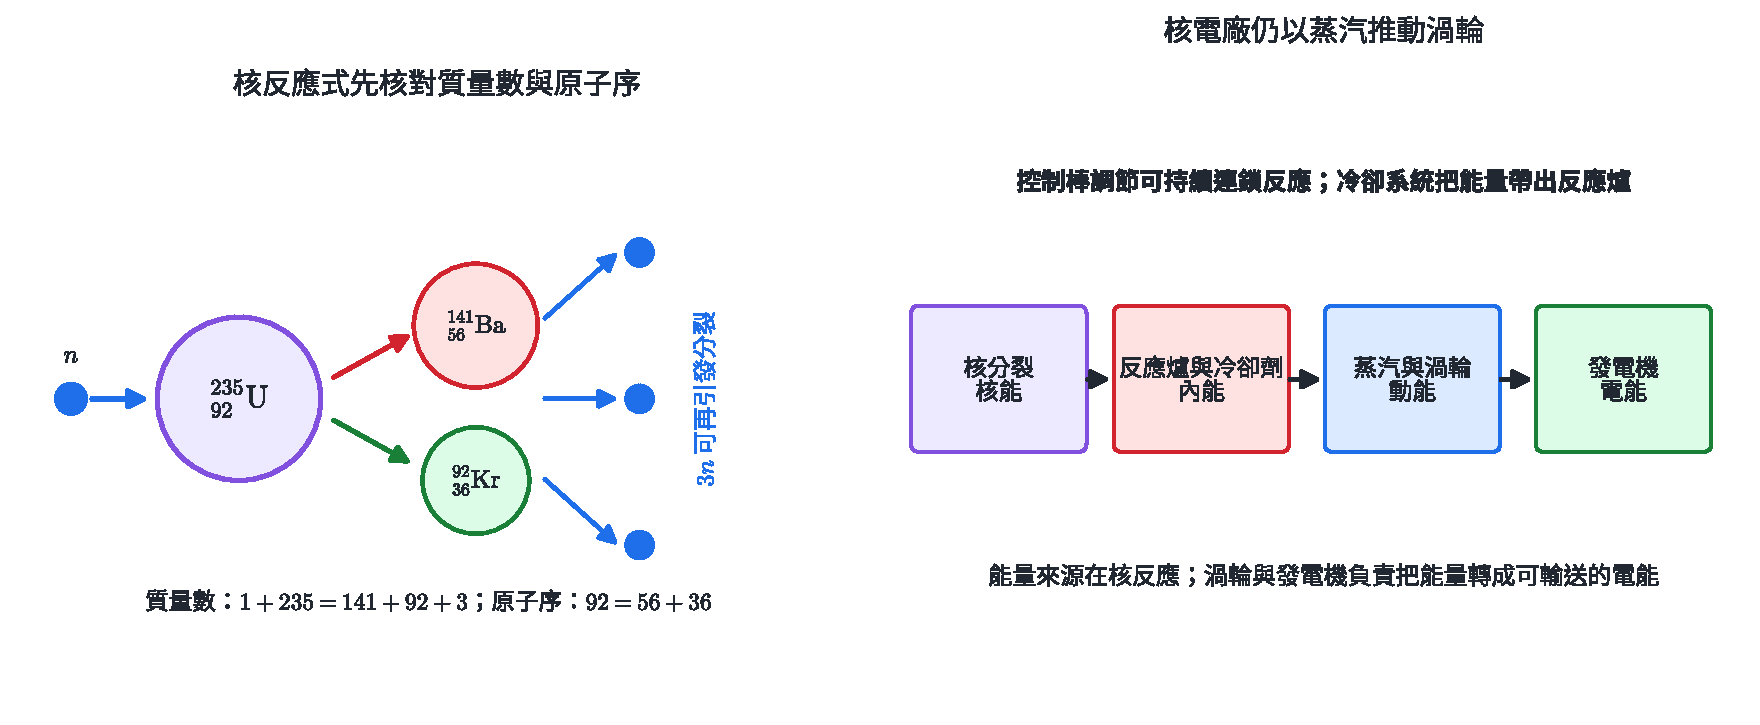
\includegraphics[keepaspectratio,alt={核分裂連鎖反應與核能發電}]{assets/必物-5-核分裂連鎖與發電.pdf}}
\caption{核分裂連鎖反應與核能發電}
\end{figure}

重原子核吸收中子後可分裂成較輕的原子核並放出中子與能量。圖中的一個示例為

\[
{}^1_0n+{}^{235}_{92}\mathrm U
\rightarrow{}^{141}_{56}\mathrm{Ba}
+{}^{92}_{36}\mathrm{Kr}+3{}^1_0n+E.
\]

質量數：\(1+235=141+92+3\)；原子序：\(0+92=56+36\)。釋出的中子可引發其他原子核分裂，形成連鎖反應。反應爐以控制棒吸收部分中子，使反應速率維持可控制；冷卻系統把內能帶出反應爐。

核能發電的主轉換鏈為

\[
\text{核能}\rightarrow\text{內能}\rightarrow
\text{蒸汽與渦輪動能}\rightarrow\text{電能}.
\]

核燃料能量密度高，運轉階段的直接溫室氣體排放較低；燃料開採、建廠、除役、放射性廢棄物與事故風險也須納入整體評估。

\subsubsection{示範 15　補全核反應式}\label{ux793aux7bc4-15-ux88dcux5168ux6838ux53cdux61c9ux5f0f}

\[
{}^1_0n+{}^{235}_{92}\mathrm U
\rightarrow{}^{144}_{56}\mathrm{Ba}
+{}^{89}_{Z}\mathrm X+3{}^1_0n.
\]

由原子序守恆：\(92=56+Z\)，得 \(Z=36\)，所以 X 是 Kr。質量數核對：\(1+235=144+89+3=236\)。完整產物為 \({}^{89}_{36}\mathrm{Kr}\)。

\subsection{4.3 游離輻射與安全}\label{ux6e38ux96e2ux8f3bux5c04ux8207ux5b89ux5168}

\begin{figure}
\centering
\pandocbounded{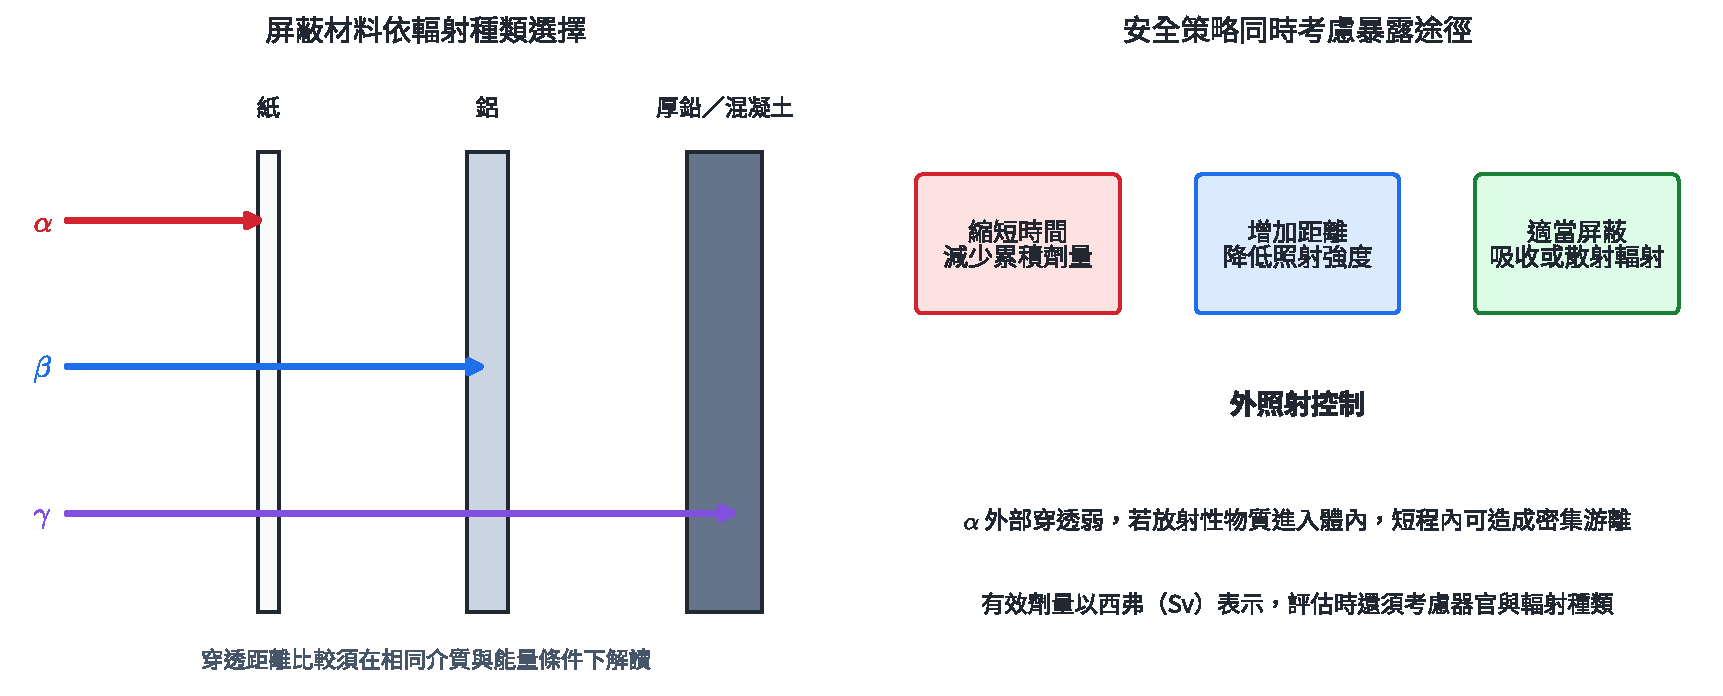
\includegraphics[keepaspectratio,alt={游離輻射、穿透與安全策略}]{assets/必物-5-游離輻射與屏蔽.pdf}}
\caption{游離輻射、穿透與安全策略}
\end{figure}

游離輻射能使物質中的原子或分子失去電子。核衰變常見的三類輻射為：

{\def\LTcaptype{none} % do not increment counter
\begin{longtable}[]{@{}
  >{\raggedright\arraybackslash}p{(\linewidth - 6\tabcolsep) * \real{0.2308}}
  >{\raggedright\arraybackslash}p{(\linewidth - 6\tabcolsep) * \real{0.2308}}
  >{\raggedleft\arraybackslash}p{(\linewidth - 6\tabcolsep) * \real{0.3077}}
  >{\raggedright\arraybackslash}p{(\linewidth - 6\tabcolsep) * \real{0.2308}}@{}}
\toprule\noalign{}
\begin{minipage}[b]{\linewidth}\raggedright
類型
\end{minipage} & \begin{minipage}[b]{\linewidth}\raggedright
本質
\end{minipage} & \begin{minipage}[b]{\linewidth}\raggedleft
電荷
\end{minipage} & \begin{minipage}[b]{\linewidth}\raggedright
典型穿透與屏蔽
\end{minipage} \\
\midrule\noalign{}
\endhead
\bottomrule\noalign{}
\endlastfoot
\(\alpha\) & 氦原子核 \({}^4_2\mathrm{He}\) & \(+2e\) & 空氣中射程短，紙或皮膚表層可阻擋 \\
\(\beta^-\) & 高速電子 & \(-e\) & 可穿過紙，常以適當厚度的塑膠或鋁屏蔽 \\
\(\gamma\) & 高能電磁波 & 0 & 穿透較強，以厚鉛或混凝土降低強度 \\
\end{longtable}
}

穿透力與游離密度是兩個不同指標。\(\alpha\) 外照射常被皮膚表層阻擋；若放射性物質經呼吸或飲食進入體內，短射程內的密集游離會增加局部組織風險。

有效劑量單位為西弗（Sv），用來把吸收能量、輻射種類與組織敏感度納入風險尺度。外照射的基本控制是縮短時間、增加距離、使用合適屏蔽；污染控制還包括阻止放射性物質進入人體。

\subsubsection{示範 16　選擇屏蔽與操作方式}\label{ux793aux7bc4-16-ux9078ux64c7ux5c4fux853dux8207ux64cdux4f5cux65b9ux5f0f}

實驗需短時間操作密封的 \(\gamma\) 射源。合理控制包括：先規劃步驟以縮短近源時間，使用夾具增加手與射源的距離，並把射源置於經設計的鉛屏蔽內。三項措施分別作用於暴露時間、到源距離與穿透衰減，彼此可以同時使用。

\subsection{4.4 核融合}\label{ux6838ux878dux5408}

\begin{figure}
\centering
\pandocbounded{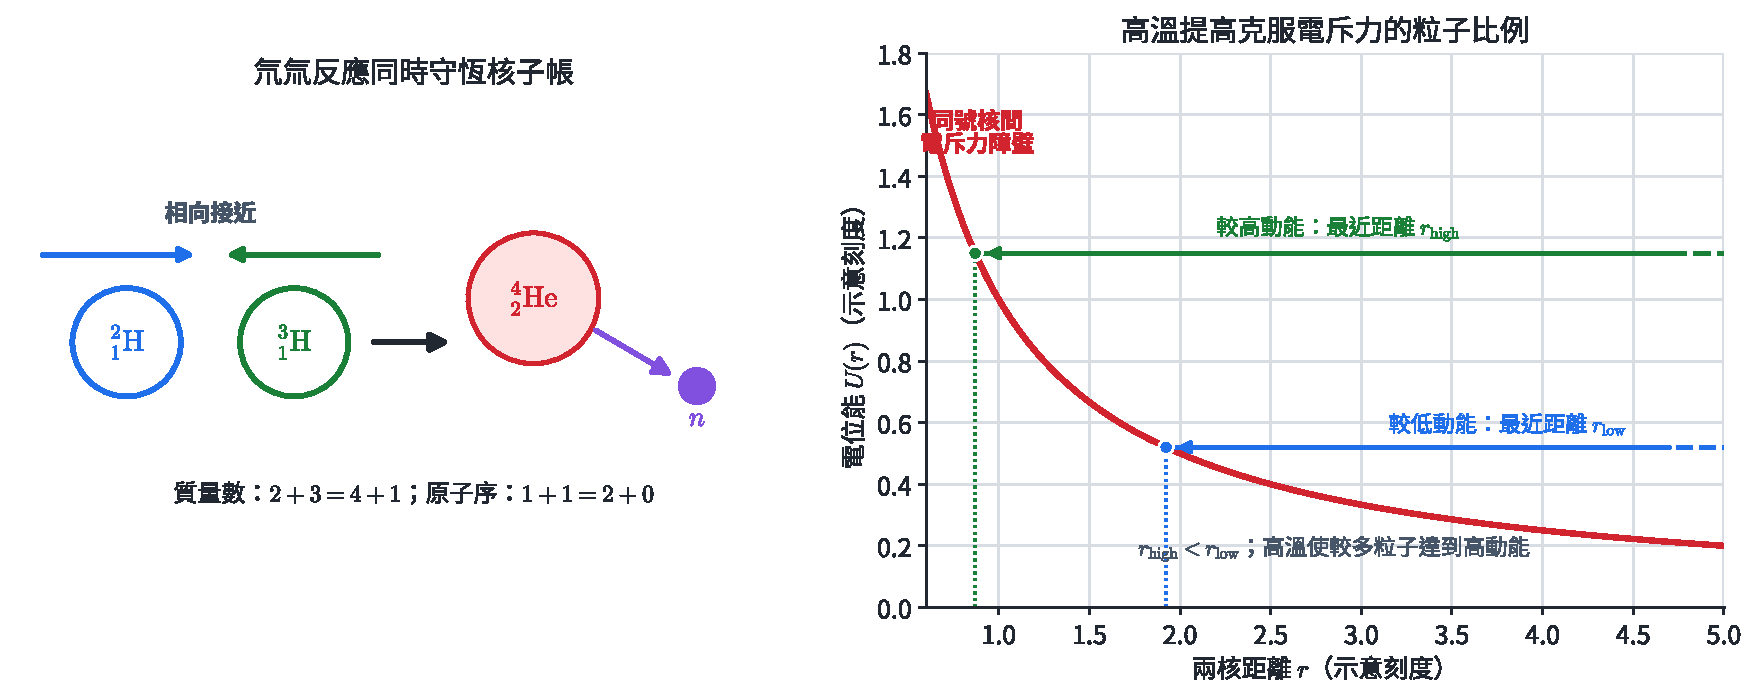
\includegraphics[keepaspectratio,alt={氘核與氚核相向接近並融合；較高動能使兩核能到達更小的最近距離}]{assets/必物-5-核融合反應與高溫條件.pdf}}
\caption{氘核與氚核相向接近並融合；較高動能使兩核能到達更小的最近距離}
\end{figure}

輕原子核結合成較重原子核的過程稱為核融合。氘氚反應可寫成

\[
{}^2_1\mathrm H+{}^3_1\mathrm H
\rightarrow{}^4_2\mathrm{He}+{}^1_0n+E.
\]

質量數 \(2+3=4+1\)，原子序 \(1+1=2+0\)。兩個原子核皆帶正電，接近時需克服電斥力；約 \(10^8\ \mathrm K\) 的高溫可使較多粒子具有足夠動能接近到核力能發揮作用的距離。太陽核心以高溫與巨大重力約束維持融合。地面裝置還需同時處理高溫電漿約束、材料受中子照射、能量取出與持續穩定運轉等工程問題。

\subsubsection{示範 17　融合反應的核子帳}\label{ux793aux7bc4-17-ux878dux5408ux53cdux61c9ux7684ux6838ux5b50ux5e33}

考慮

\[
{}^2_1\mathrm H+{}^2_1\mathrm H
\rightarrow{}^3_2\mathrm{He}+X.
\]

質量數：\(2+2=3+A_X\)，所以 \(A_X=1\)。原子序：\(1+1=2+Z_X\)，所以 \(Z_X=0\)。因此 \(X={}^1_0n\)。

\subsection{本節練習}\label{ux672cux7bc0ux7df4ux7fd2-3}

\begin{enumerate}
\def\labelenumi{\arabic{enumi}.}
\tightlist
\item
  \(1.0\times10^{-9}\ \mathrm{kg}\) 的質量差對應多少能量？
\item
  在 \({}^{A}_{Z}\mathrm X\) 中，\(A\) 與 \(Z\) 各代表什麼？中子數如何表示？
\item
  補全：\({}^{238}_{92}\mathrm U\rightarrow{}^{234}_{90}\mathrm{Th}+X\)。
\item
  依序寫出核能電廠從核分裂到輸出電能的主要能量形式。
\item
  分別為 \(\alpha\)、\(\beta\)、\(\gamma\) 選擇紙、鋁、厚鉛／混凝土三種典型屏蔽，並指出增加距離主要降低哪一項暴露因素。
\item
  核融合需要高溫的微觀原因為何？核對氘氚反應的質量數與原子序。
\end{enumerate}

答案：1. \(9.0\times10^7\ \mathrm J\)。2. \(A\) 為質量數，\(Z\) 為原子序；中子數 \(A-Z\)。3. \({}^4_2\mathrm{He}\)，即 \(\alpha\) 粒子。4. 核能、內能、蒸汽與渦輪動能、電能。5. 紙---\(\alpha\)，鋁---\(\beta\)，厚鉛／混凝土---\(\gamma\)；增加距離降低到達人體的照射強度。6. 增加具有足夠動能克服核間電斥力的粒子比例；\(A:2+3=4+1\)，\(Z:1+1=2+0\)。

\section{5　章末代表題}\label{ux7ae0ux672bux4ee3ux8868ux984c}

\subsection{A　核心模型與單一情境}\label{a-ux6838ux5fc3ux6a21ux578bux8207ux55aeux4e00ux60c5ux5883}

\begin{enumerate}
\def\labelenumi{\arabic{enumi}.}
\item
  \textbf{常力作功}　人以 \(40\ \mathrm N\) 的力拉箱子，拉力與水平位移夾 \(60^\circ\)，箱子水平移動 \(5.0\ \mathrm m\)。求拉力作功。
\item
  \textbf{力---位置圖}　某物體所受沿 \(x\) 方向的合力，在 \(x=0\) 到 \(2.0\ \mathrm m\) 間由 \(0\) 線性增加到 \(6.0\ \mathrm N\)，在 \(x=2.0\) 到 \(5.0\ \mathrm m\) 間維持 \(6.0\ \mathrm N\)。求合力作功。
\item
  \textbf{功---動能定理}　質量 \(4.0\ \mathrm{kg}\) 的物體速率由 \(2.0\ \mathrm{m/s}\) 增至 \(6.0\ \mathrm{m/s}\)。求這段過程的合功。
\item
  \textbf{功率與效率}　升降設備在 \(20\ \mathrm s\) 內把 \(800\ \mathrm{kg}\) 的貨物等速提升 \(12\ \mathrm m\)，輸入功率為 \(6.0\ \mathrm{kW}\)。取 \(g=10\ \mathrm{m/s^2}\)，求有用輸出功率與效率。
\item
  \textbf{平均動能與內能}　同種理想氣體 A 有 \(N\) 個粒子、溫度 \(300\ \mathrm K\)；B 有 \(2N\) 個粒子、溫度 \(450\ \mathrm K\)。求 B 與 A 的平均分子動能比及總內能比。
\item
  \textbf{絕對溫度}　某理想氣體初溫為 \(27^\circ\mathrm C\)。若平均分子動能變為三倍，末溫約為多少 \(^\circ\mathrm C\)？
\item
  \textbf{力學能守恆}　物體在光滑軌道 A 點高度 \(7.0\ \mathrm m\)、速率 \(4.0\ \mathrm{m/s}\)，移到高度 \(2.0\ \mathrm m\) 的 B 點。取 \(g=10\ \mathrm{m/s^2}\)，求 B 點速率。
\item
  \textbf{摩擦與熱能}　\(2.0\ \mathrm{kg}\) 滑塊由高 \(5.0\ \mathrm m\) 處靜止下滑，到達零位面時速率為 \(6.0\ \mathrm{m/s}\)。取 \(g=10\ \mathrm{m/s^2}\)，求滑塊與斜面增加的熱能。
\item
  \textbf{量熱與效率}　\(600\ \mathrm W\) 加熱器以 \(75\%\) 效率加熱 \(0.30\ \mathrm{kg}\) 的水，使水升溫 \(25^\circ\mathrm C\)。取 \(c=4200\ \mathrm{J/(kg\cdot{}^\circ C)}\)，求所需時間。
\item
  \textbf{多段能量轉換}　裝置三段效率依序為 \(80\%\)、\(70\%\)、\(90\%\)，輸入能量為 \(2.0\ \mathrm{MJ}\)。求總效率、有用輸出與流向環境的能量。
\item
  \textbf{質能關係}　核反應前後總質量減少 \(5.0\times10^{-12}\ \mathrm{kg}\)。求釋放能量。
\item
  \textbf{核反應與輻射}　核分裂反應

  \[
  {}^1_0n+{}^{235}_{92}\mathrm U
  \rightarrow{}^{140}_{54}\mathrm{Xe}
  +{}^{94}_{38}\mathrm{Sr}+x{}^1_0n
  \]

  求 \(x\)。若反應產物伴隨強 \(\gamma\) 輻射，指出適合的屏蔽材料；再說明 \(\alpha\) 放射性物質進入體內時須重視的原因。
\end{enumerate}

\subsection{B　跨節整合題}\label{b-ux8de8ux7bc0ux6574ux5408ux984c}

\begin{enumerate}
\def\labelenumi{\arabic{enumi}.}
\setcounter{enumi}{12}
\item
  \textbf{起重機：功、機械能、功率與效率}　起重機把 \(600\ \mathrm{kg}\) 貨物由靜止提升 \(15\ \mathrm m\)，末速率為 \(5.0\ \mathrm{m/s}\)，全程 \(30\ \mathrm s\)。起重機效率為 \(75\%\)，取 \(g=10\ \mathrm{m/s^2}\)。求貨物與地球系統的機械能增加量、起重機輸入能量與輸入功率。
\item
  \textbf{雲霄飛車：位能、動能、摩擦熱與煞車}　\(500\ \mathrm{kg}\) 車廂由高 \(20\ \mathrm m\) 處靜止出發，到達高 \(5.0\ \mathrm m\) 的平台入口時速率為 \(8.0\ \mathrm{m/s}\)。車廂隨後在同一高度煞停。取 \(g=10\ \mathrm{m/s^2}\)。求第一段摩擦造成的熱能增加、煞車段的熱能增加，以及從出發到停止的總熱能增加。
\item
  \textbf{核電廠：質能、效率與功率}　某核電機組輸出電功率 \(900\ \mathrm{MW}\)，核能到電能的整體效率為 \(36\%\)。每次核分裂的質量虧損為 \(3.2\times10^{-28}\ \mathrm{kg}\)。假設輸出維持 \(1.0\ \mathrm h\)，求所需核反應釋放能量、約發生多少次分裂，以及這些反應的總質量虧損。並寫出反應能到電能的主要轉換鏈。
\item
  \textbf{抽蓄儲能：效率、功率與質能尺度}　抽蓄系統在充電時輸入 \(5.0\times10^{10}\ \mathrm J\)，往返效率為 \(68\%\)。放電期間平均輸出功率為 \(20\ \mathrm{MW}\)。求可回收電能、可維持輸出的時間，以及這筆回收能量所對應的質量 \(E/c^2\)。
\end{enumerate}

\section{6　章末題完整詳解}\label{ux7ae0ux672bux984cux5b8cux6574ux8a73ux89e3}

\subsection{第 1 題}\label{ux7b2c-1-ux984c}

位移水平向前，與拉力夾角已知，使用常力功：

\[
W=Fs\cos\theta=(40)(5.0)\cos60^\circ=100\ \mathrm J.
\]

拉力含有沿位移的正向分量，所以功為正。

\subsection{第 2 題}\label{ux7b2c-2-ux984c}

合功等於 \(F_x-x\) 圖的面積。前段是三角形，後段是矩形：

\[
W=\frac12(2.0)(6.0)+(5.0-2.0)(6.0)
=6.0+18=24\ \mathrm J.
\]

兩段都在橫軸上方，面積皆取正。

\subsection{第 3 題}\label{ux7b2c-3-ux984c}

使用功---動能定理：

\[
W_{\mathrm{net}}=\Delta K
=\frac12m(v_f^2-v_i^2)
=\frac12(4.0)(6.0^2-2.0^2)
=64\ \mathrm J.
\]

末速率較大，動能增加，合功為正。

\subsection{第 4 題}\label{ux7b2c-4-ux984c}

貨物等速上升，動能不變，有用輸出是增加的重力位能：

\[
\Delta U_g=mgh=(800)(10)(12)=9.6\times10^4\ \mathrm J.
\]

有用輸出功率：

\[
P_{\mathrm{useful}}=\frac{9.6\times10^4}{20}
=4.8\times10^3\ \mathrm W=4.8\ \mathrm{kW}.
\]

效率：

\[
\eta=\frac{4.8}{6.0}=0.80=80\%.
\]

\subsection{第 5 題}\label{ux7b2c-5-ux984c}

理想氣體平均分子動能與絕對溫度成正比：

\[
\frac{\overline K_B}{\overline K_A}
=\frac{450}{300}=1.5.
\]

總內能還與粒子數成正比：

\[
\frac{U_B}{U_A}
=\frac{(2N)(450)}{N(300)}=3.0.
\]

B 的平均分子動能為 A 的 \(1.5\) 倍，總內能為 A 的 \(3.0\) 倍。

\subsection{第 6 題}\label{ux7b2c-6-ux984c}

先轉為絕對溫度：\(27^\circ\mathrm C\approx300\ \mathrm K\)。平均動能成為三倍，因此

\[
T_f=3(300)=900\ \mathrm K.
\]

轉回攝氏：

\[
t_f=900-273.15=626.85^\circ\mathrm C
\approx627^\circ\mathrm C.
\]

\subsection{第 7 題}\label{ux7b2c-7-ux984c}

軌道光滑，以物體與地球為系統，機械能守恆：

\[
\frac12mv_A^2+mgh_A
=\frac12mv_B^2+mgh_B.
\]

質量約去：

\[
v_B^2=v_A^2+2g(h_A-h_B)
=4.0^2+2(10)(7.0-2.0)=116.
\]

\[
v_B=\sqrt{116}\approx10.8\ \mathrm{m/s}.
\]

B 較低，重力位能下降並轉為動能，末速率大於初速率。

\subsection{第 8 題}\label{ux7b2c-8-ux984c}

滑塊與地球、斜面合為系統。初態只有重力位能：

\[
E_i=mgh=(2.0)(10)(5.0)=100\ \mathrm J.
\]

到零位面時的動能：

\[
K_f=\frac12mv^2=\frac12(2.0)(6.0)^2=36\ \mathrm J.
\]

總能量守恆，差值成為熱能：

\[
\Delta E_{\mathrm{th}}=100-36=64\ \mathrm J.
\]

\subsection{第 9 題}\label{ux7b2c-9-ux984c}

水所需能量：

\[
Q=mc\Delta T=(0.30)(4200)(25)=3.15\times10^4\ \mathrm J.
\]

加熱器的有用功率：

\[
P_{\mathrm{useful}}=\eta P_{\mathrm{in}}=0.75(600)=450\ \mathrm W.
\]

所需時間：

\[
t=\frac{Q}{P_{\mathrm{useful}}}
=\frac{3.15\times10^4}{450}=70\ \mathrm s.
\]

\subsection{第 10 題}\label{ux7b2c-10-ux984c}

總效率是逐段效率相乘：

\[
\eta_{\mathrm{total}}=(0.80)(0.70)(0.90)=0.504=50.4\%.
\]

有用輸出：

\[
E_{\mathrm{useful}}=0.504(2.0\ \mathrm{MJ})
=1.008\ \mathrm{MJ}.
\]

流向環境的能量為

\[
E_{\mathrm{env}}=2.0-1.008=0.992\ \mathrm{MJ}.
\]

輸出與環境所得相加為原輸入 \(2.0\ \mathrm{MJ}\)。

\subsection{第 11 題}\label{ux7b2c-11-ux984c}

\[
E=\Delta mc^2
=(5.0\times10^{-12})(3.0\times10^8)^2
=4.5\times10^5\ \mathrm J.
\]

\subsection{第 12 題}\label{ux7b2c-12-ux984c}

先核對原子序：\(92=54+38\)，已平衡。質量數守恆給出

\[
1+235=140+94+x,
\]

所以 \(236=234+x\)，得 \(x=2\)。

\(\gamma\) 穿透力較強，典型屏蔽採用足夠厚度的鉛或混凝土。\(\alpha\) 粒子在物質中射程短、游離密度高；放射性物質進入體內後，能量可集中沉積於鄰近組織，因此須控制吸入與攝入。

\subsection{第 13 題}\label{ux7b2c-13-ux984c}

選貨物與地球為系統。起重機輸入的有用機械能同時增加重力位能與動能：

\[
\Delta U_g=mgh=(600)(10)(15)=9.0\times10^4\ \mathrm J,
\]

\[
\Delta K=\frac12mv_f^2
=\frac12(600)(5.0)^2=7.5\times10^3\ \mathrm J.
\]

因此

\[
\Delta E_{\mathrm{mech}}=9.75\times10^4\ \mathrm J.
\]

效率 \(\eta=E_{\mathrm{useful}}/E_{\mathrm{in}}\)，所以

\[
E_{\mathrm{in}}=\frac{9.75\times10^4}{0.75}
=1.30\times10^5\ \mathrm J.
\]

輸入功率為

\[
P_{\mathrm{in}}=\frac{E_{\mathrm{in}}}{t}
=\frac{1.30\times10^5}{30}
\approx4.33\times10^3\ \mathrm W=4.33\ \mathrm{kW}.
\]

機械能增加量除以時間為有用功率 \(3.25\ \mathrm{kW}\)，也等於 \(0.75P_{\mathrm{in}}\)。

\subsection{第 14 題}\label{ux7b2c-14-ux984c}

把車廂、地球與軌道合為系統，以地面為零位面。出發時總機械能：

\[
E_i=mgh_i=(500)(10)(20)=1.00\times10^5\ \mathrm J.
\]

平台入口的重力位能與動能為

\[
U_1=(500)(10)(5.0)=2.50\times10^4\ \mathrm J,
\]

\[
K_1=\frac12(500)(8.0)^2=1.60\times10^4\ \mathrm J.
\]

第一段末機械能為 \(4.10\times10^4\ \mathrm J\)，所以第一段熱能增加

\[
\Delta E_{{\mathrm{th}},1}=1.00\times10^5-4.10\times10^4
=5.90\times10^4\ \mathrm J.
\]

煞車時高度不變，動能 \(1.60\times10^4\ \mathrm J\) 全部轉為熱能：

\[
\Delta E_{{\mathrm{th}},2}=1.60\times10^4\ \mathrm J.
\]

總熱能增加：

\[
\Delta E_{\mathrm{th},total}=5.90\times10^4+1.60\times10^4
=7.50\times10^4\ \mathrm J.
\]

停止時只剩 \(2.50\times10^4\ \mathrm J\) 重力位能，與初能量差同樣是 \(7.50\times10^4\ \mathrm J\)。

\subsection{第 15 題}\label{ux7b2c-15-ux984c}

輸出電功率 \(P_e=900\ \mathrm{MW}=9.00\times10^8\ \mathrm W\)。效率為

\[
\eta=\frac{E_e}{E_{\mathrm{nuclear}}}=0.36.
\]

一小時輸出的電能為

\[
E_e=P_et=(9.00\times10^8)(3600)
=3.24\times10^{12}\ \mathrm J.
\]

所需反應能：

\[
E_{\mathrm{nuclear}}=\frac{3.24\times10^{12}}{0.36}
=9.00\times10^{12}\ \mathrm J.
\]

每次分裂釋放的能量：

\[
E_1=(3.2\times10^{-28})(3.0\times10^8)^2
=2.88\times10^{-11}\ \mathrm J.
\]

分裂次數：

\[
N=\frac{9.00\times10^{12}}{2.88\times10^{-11}}
\approx3.13\times10^{23}.
\]

總質量虧損可由 \(N\Delta m_1\) 或 \(E/c^2\) 求得：

\[
\Delta m=N(3.2\times10^{-28})
\approx1.00\times10^{-4}\ \mathrm{kg}=0.100\ \mathrm g.
\]

主要轉換鏈為核分裂釋放的核能 \(\rightarrow\) 反應爐與冷卻劑的內能 \(\rightarrow\) 蒸汽與渦輪的動能 \(\rightarrow\) 發電機輸出的電能。效率 \(36\%\) 表示其餘能量主要由冷卻系統與環境帶走。

\subsection{第 16 題}\label{ux7b2c-16-ux984c}

可回收電能：

\[
E_{\mathrm{out}}=0.68(5.0\times10^{10})
=3.4\times10^{10}\ \mathrm J.
\]

輸出功率 \(20\ \mathrm{MW}=2.0\times10^7\ \mathrm W\)，可維持時間：

\[
t=\frac{E_{\mathrm{out}}}{P}
=\frac{3.4\times10^{10}}{2.0\times10^7}
=1.7\times10^3\ \mathrm s
\approx28\ \mathrm{min}.
\]

以質能關係換算這筆能量的等效質量尺度：

\[
m_{\mathrm{eq}}=\frac{E}{c^2}
=\frac{3.4\times10^{10}}{9.0\times10^{16}}
\approx3.8\times10^{-7}\ \mathrm{kg}
=0.38\ \mathrm{mg}.
\]

抽蓄系統實際儲存的是水的重力位能；最後一項只用來比較能量與質量的數值尺度。

\section{7　核心整理}\label{ux6838ux5fc3ux6574ux7406}

\begin{enumerate}
\def\labelenumi{\arabic{enumi}.}
\tightlist
\item
  功是力透過位移轉移的能量：恆力用 \(W=Fs\cos\theta\)，變力用 \(F_x-x\) 圖的帶號面積。
\item
  合功改變動能：\(W_{\mathrm{net}}=\Delta K\)。近地面重力位能為 \(U_g=mgh\)，零位面改變不影響位能差。
\item
  只有重力或理想彈力在系統內轉換時，\(K+U\) 守恆；摩擦使部分機械能轉成熱能，總能量仍守恆。
\item
  溫度反映粒子平均動能，內能是系統微觀能量的總和。理想氣體平均動能的倍數關係以克氏溫標判讀。
\item
  熱是因溫差傳遞的能量；無相變且比熱固定時，\(Q=mc\Delta T\)。功率描述轉換速率，效率描述有用輸出比例。
\item
  核反應先核對質量數與原子序，再以 \(E=\Delta mc^2\) 連接質量虧損與釋放能量。
\item
  輻射安全依種類與暴露途徑選擇時間、距離、屏蔽與污染控制；融合的高溫條件源自帶正電原子核間的電斥力。
\end{enumerate}


\end{document}
